\documentclass[10pt]{article}

\usepackage[margin=0.85in]{geometry}
\usepackage[T1]{fontenc}
\usepackage{lmodern}
\usepackage{microtype}
\usepackage{graphicx}
\usepackage{booktabs}
\usepackage{array}
\usepackage{multirow}
\usepackage{amsmath,amssymb}
\usepackage{enumitem}
\usepackage[dvipsnames]{xcolor}
\usepackage[round,authoryear]{natbib}
\usepackage[colorlinks=true,allcolors=MidnightBlue]{hyperref}
\usepackage[nameinlink,noabbrev]{cleveref}
\usepackage{url}

\setlist{nosep}
\graphicspath{{figures/}}
\hypersetup{
  pdftitle={GAWorld v2: A Configurable Research Stack for LLM-Based Artificial Societies},
  pdfauthor={Author Name(s)},
  pdfsubject={LLM-based artificial societies, multi-agent social simulation, research infrastructure},
  pdfkeywords={LLM agents, multi-agent systems, artificial societies, social simulation, research infrastructure, parallel worlds, agent-based modeling}
}

\title{GAWorld v2: A Configurable Research Stack for LLM-Based Artificial Societies}

\author{Author Name(s)\\Affiliation(s)\\\texttt{email@example.org}}

\date{2026}

\begin{document}
\maketitle

\begin{abstract}
LLM agents make it possible to study social interaction through profiles, plans,
and language, yet most demonstrations stop at a single transcript or a small
isolated scenario.  Research on society-level questions needs persistent
inhabitants whose state, memory, relationships, and exposure change across
simulated time; a shared urban and institutional substrate; explicit
intervention points; configurable deployments for one researcher, a classroom,
or a distributed cluster; and an evidence layer that records what was run, what
completed, and what did not.  We present GAWorld v2, a research stack that
integrates these concerns.  v2 adds a 14-plugin microkernel, per-tenant world
isolation, distributed execution over many machines, a parallel-worlds
counterfactual engine, an Agent Playground of fourteen game-based probes, a
Research Workbench for paper-to-protocol compilation, an Agent Arena for
LLM-resident benchmarking, persona distillation from real people, and
endogenous economics, indoor spatial reasoning, organizational governance, and
audited hooks for offline citizens.  The system is engineered as a configurable
instrument rather than a calibrated population model: every capability is
traceable to a built-in plugin, an event-bus contribution, or a documented
compatibility path, and every reported number in the present paper is bound to
a hashed artifact whose evidence class is explicit.  We describe the
architecture, audit representative capabilities against their evidence class,
and state the validation, reproducibility, and ethical boundaries that govern
intended use.  GAWorld v2 does not validate an artificial city; it makes the
construction, audit, and revision of artificial-society experiments tractable.
\end{abstract}

\section{Introduction}
\label{sec:introduction}

Large language models have made it possible to construct agents that read
natural-language situations, plan, and write socially legible actions.  This
capability has renewed interest in \emph{generative agents} and in
\emph{LLM-based social simulation}
\citep{park2023generative,park2024grounded,argyle2023outofone}, but a
persuasive conversation is not yet an artificial society.  A research-grade
artificial society must let its inhabitants persist across simulated time, act
from shared locations and relations, encounter consequences of earlier
decisions, and leave evidence from which a researcher can reconstruct what
happened.  The mechanisms that surround the language model---time, space,
exposure, institutions, resource constraints, audit, and intervention---must
be explicit enough to inspect and vary.  This is a systems problem, not a
prompt-crafting problem.

GAWorld is research infrastructure for building such societies.  The first
arXiv system paper froze the audited K1--K5 microkernel state of the codebase
at a single repository commit and reported nine built-in plugins, an artifact
ledger, and a single-tenant, single-process deployment model
\citep{gawoerldv1}.  Since that snapshot, the system has been extended in five
directions that, taken together, change what the platform is for:

\begin{enumerate}[leftmargin=*,label=\textbf{\arabic*.}]
  \item \textbf{Plugin breadth and surface closure.}  The built-in plugin set
  has grown from nine to fourteen; new plugins add personality-grounded
  behavior, dynamic interruption rules, indoor room resolution, an
  information-diet that mixes agent-derived queries with external sources, and
  organizational governance.  Each plugin either participates through the
  event bus or is admitted as a built-in whose semantics are documented.
  \item \textbf{Multi-tenant worlds.}  A persistent account store with
  invite-code registration, role-based membership, per-world configuration
  overlays, copy-on-write city bundles, per-tenant quotas, and audit trails
  lets a single deployment host many independent societies with different
  visibility.  When the account store is absent the system reverts, byte for
  byte, to its single-tenant behavior.
  \item \textbf{Distributed execution and playable cities.}  A world may be
  partitioned across a hub and many nodes: the hub owns accounts, the world
  metadata, and the players; each node runs its assigned inhabitants with its
  own model key.  Players can enter an \emph{open} world through a browser
  lease, claim a resident, and act in the next tick; a strict intervention
  outbox routes their actions to the right node.  This is a deployment
  primitive, not a claim of high-throughput distributed simulation.
  \item \textbf{Research and counterfactual workflow.}  Beyond the
  matched-event workflow, the stack adds a parallel-worlds engine that runs up
  to eight matched worlds across multiple seeds, a Research Workbench that
  compiles a paper or research idea into a pre-registered protocol, an
  Agent Arena for benchmarking residents, a policy simulation and optimization
  loop, and a serious-game workshop.  Each result is bound to a hash, a
  record of completion, and an evidence class.
  \item \textbf{Persona distillation and population work.}  A name or a URL
  can be distilled into a sourced portrait that becomes a resident plus a
  reusable mental-model skill; offline citizens, families, organizations, and
  bulk imports now coexist with online ones.  The City API and Agent Studio
  expose population construction as a first-class activity.
\end{enumerate}

The platform has also internalized the lessons of its first audit.  Where
v1 distinguished implementation visibility from empirical validity, v2 adds
explicit evidence classes (\textsf{REAL}, \textsf{DIAGNOSTIC},
\textsf{SYNTHETIC}, \textsf{INCOMPLETE}, \textsf{DESIGNED}, \textsf{FIXTURE}) and
insists that every reported number carry an evidence class and a hash.  Where
v1 described a single notebook, v2 separates a self-contained harness
(\textsf{GAWorld-Bench Track~A}, software-path diagnostics) from a gameplay
probe library (\textsf{Track~B}, judgement-based evaluation).  Where v1
described a single, frozen migration, v2 describes an open engineering frontier
together with the current migration status of each subsystem.

This paper makes five contributions:

\begin{enumerate}[leftmargin=*,label=\textbf{C\arabic*.}]
  \item \textbf{An integrated, plugin-bounded research stack.}  We describe
  the v2 architecture, the boundary between the kernel and the
  domain-owned plugins, and the event-bus semantics that lets mechanisms
  observe, contribute, and filter at defined lifecycles.  The architecture
  covers 14 built-in plugins, an agent step pipeline of 12 stages, a
  per-tenant world path resolver, a distributed hub-and-node protocol, and a
  parallel-worlds engine.

  \item \textbf{Multi-tenant, multi-machine, playable societies.}  We show how
  a single deployment hosts a classroom, a research group, and a
  cross-machine run from the same codebase, with per-world isolation,
  per-tenant quotas, role-based visibility, and a hub-node message relay that
  routes player interventions to the correct node in at most one tick.

  \item \textbf{An inspectable, evidence-classed experimental workflow.}  We
  integrate matched-event, parallel-worlds, paper-to-protocol, policy
  optimization, and gameplay-based evaluation under a single evidence ledger
  with hash-bound artifacts.  Each research question has a permitted claim
  class, and each numerical result carries the evidence class and the
  producing code path.

  \item \textbf{Behavior realism and societal substrate.}  We describe the
  persistent state, the Big-Five personality plugin, the dynamic-interruption
  module, the spatial tree that brings indoor rooms into the simulation, the
  endogenous inflation and credit-bound consumption model, the
  organizational-governance engine, and the offline-resident taxonomy.

  \item \textbf{Validation, reproducibility, and ethical boundaries.}  We
  report the same five-claim validation framework as v1, expanded to
  accommodate the new evidence classes and the new research surfaces, and
  we map the engineering and research roadmaps onto the boundary between
  software progress and substantive social-scientific claim.
\end{enumerate}

\begin{figure}[t]
  \centering
  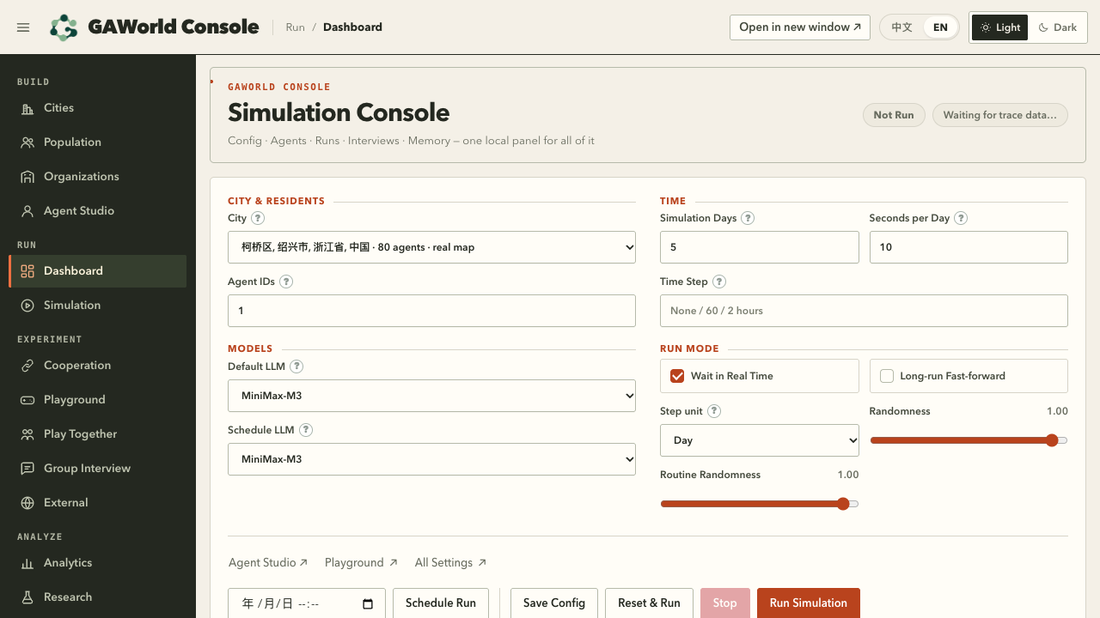
\includegraphics[width=\linewidth]{en_01_console.png}
  \caption{The GAWorld Console.  The left navigation exposes every
  v2 surface: \emph{Cities} and \emph{Population} build the city bundle;
  \emph{Organizations} edits rules and members; \emph{Agent Studio} shapes
  individual residents; the \emph{Dashboard} (shown) configures and starts a
  run; the \emph{Playground}, \emph{Play Together}, and \emph{Group Interview}
  tabs run game-based probes, an open-world player lease, and one-shot
  elicitation; \emph{External} drives the relay and external-environment
  services; and \emph{Analytics} / \emph{Research} surface the result
  inspection and the counterfactual / paper-to-protocol workflows.  The
  screenshot was captured against the bundled Keqiao (Shaoxing) city bundle
  in single-tenant, single-process mode; the dashboard UI was switched to
  English via \texttt{window.setLocale('en')}, while the resident content
  reflects the language of the bundled data.}
  \label{fig:console}
\end{figure}

GAWorld v2 is presented as a configurable scientific instrument, not as a
representative synthetic population, a digital twin, or a forecasting
system.  Its artifacts do not establish that generated agents reproduce
particular people, that aggregate trajectories match a real city, or that a
simulated intervention estimates a real policy effect.  We instead treat the
system as an instrument whose outputs are evaluated at five claim levels
(individual consistency, macro correspondence, emergent dynamics,
counterfactual response, reproducibility) and whose evidence ledger is a
prerequisite for substantive interpretation.

The remainder of the paper proceeds as follows.  \Cref{sec:design-goals}
states the design goals; \Cref{sec:related-work} positions v2 against
generative agents, language agents, social evaluation, agent-based modeling,
and platform research.  \Cref{sec:agent-lifecycle,sec:microkernel,sec:memory-cognition-realism}
describe the agent, the kernel, and the cognitive substrate.
\Cref{sec:substrate,sec:multi-user-worlds,sec:distributed-playable} describe
the societal substrate, multi-tenancy, and the distributed playable runtime.
\Cref{sec:research-workflow,sec:playground-arena} describe the research and
gameplay surfaces.  \Cref{sec:capability-cases,sec:validation-boundaries}
audit the existing capability cases against the five claim levels.
\Cref{sec:limitations-ethics-roadmap} states the limits and the roadmap.
\Cref{sec:conclusion} concludes.

\section{Design Goals}
\label{sec:design-goals}

GAWorld v2 is intended as a configurable research instrument rather than as a
claim that a language model is, by itself, a valid population model.  Its
design goals therefore concern properties that a researcher can inspect in the
running system, and each property has a concrete mechanism in the present
implementation and a boundary that prevents the mechanism from being read as an
empirical guarantee.  Where v1 listed six properties, v2 lists eight, adding
two that the v1 platform could not satisfy: \emph{per-tenant world isolation}
and \emph{human participation under the same first-class intervention surface
as scheduled events}.

\subsection{Persistence across simulated time}
\label{sec:dgo:persistence}

An agent must carry consequences from one decision context into later ones,
rather than being reconstructed from a stateless prompt at every tick.  v2
combines a mutable state record with file-backed episodic memory, daily logs
and diaries, schedules, and longer-lived relationship and growth records.  A
stateful run restores the day counter and per-agent memories; the memory
lifecycle can retrieve, consolidate, summarize, and decay stored episodes.
Persistence is therefore testable: a researcher can inspect both the state
before and after a tick and the files used in later recall.  Persistence does
not establish psychological fidelity.  Many memories and summaries are
language-model outputs, configuration can disable lifecycle operations, and
several archived cross-phase evaluations are incomplete.

\subsection{Situatedness in a shared world}
\label{sec:dgo:situatedness}

Actions should be conditioned on where and when an agent acts and on what is
locally observable.  The simulation clock exposes day, time, and tick index;
the city map represents named locations, connections, and indoor rooms; and
environment, local-physical, social, policy, and information mechanisms
contribute context to the cognition loop.  Movement updates location before
later stages use the new setting, social influence is computed over the
current network rather than over an unconstrained cast of characters, and
indoor rooms are resolved against the same activity the agent is performing.
v2's addition of an \emph{away} state \citep{gaworldtravel} lets inhabitants
temporarily leave the city and return to a specific home node.  This is
situated computation, not a calibrated digital twin: map detail, physical
dynamics, agent access to information, and the indoor-room tree are
abstractions selected by configuration.

\subsection{Composability without concealing control flow}
\label{sec:dgo:composability}

Researchers should be able to change an experimental mechanism without
rewriting the complete agent loop.  v2 provides three bounded extension
surfaces: a configurable stage sequence for cognition, an event bus with
observe/contribute/filter semantics, and a registry for lifecycle-managed
plugins.  The audited built-in set now contains fourteen plugins: intervention,
skills, interests, life events, economy, local physical perception, real
work, dynamic behavior, spatial preferences, personality, indoor rooms and
venue capacity, organizations, governance, and offline citizens.  These join
existing memory, environment, and social-network subsystems that retain direct
compatibility paths.  Each plugin declares its dependencies, owns
configuration namespaces and per-agent state, and contributes through the bus
or through lifecycle hooks.  Composability is not unrestricted hot swapping:
the stage pipeline exchanges a shared step dictionary, and three legacy
subsystems (memory, environment, social network) retain direct paths.  The
audit table in \cref{sec:microkernel} lists the boundary state of each
subsystem.

\subsection{Controllability for counterfactual experiments}
\label{sec:dgo:controllability}

A research run should expose explicit points at which a scenario or
intervention is introduced.  Configuration fixes profiles, city assets,
random seed, mechanism flags, schedules, and policy events.  The
intervention plugin contributes a recommendation feed through the event bus
and records its domain-specific metrics.  The Controller API validates
structured movement requests through a priority-ordered validator chain and
exposes audited runtime interventions for state mutation, configuration
update, and agent removal.  v2 adds three new controllability surfaces: a
parallel-worlds engine that runs up to eight matched worlds with a shared
seed; a Research Workbench that compiles a research idea or a paper into a
pre-registered protocol with pre-specified outcomes and minimum-effect
thresholds; and a policy-simulation loop that proposes a candidate policy,
simulates, scores, and iterates.  None of these are guaranteed to identify a
real-world effect; they are designed to make the construct, the contrast, and
the completion status of every arm visible to the analyst.

\subsection{Inspectability from decision to artifact}
\label{sec:dgo:inspectability}

A claim about an artificial society should be traceable to artifacts below
the level of a prose summary.  v2 writes per-agent logs and memories,
environment timelines, state histories, plugin-owned outputs, and
experiment comparisons; its interfaces expose portions of those records for
inspection and replay.  The kernel Recorder additionally implements a
clock-stamped JSONL stream and records Controller interventions and denials.
v2 adds two new inspectability surfaces: a parallel-worlds results file that
records per-arm completion status, per-resident ATE, bootstrap confidence
intervals, and sign-flip $p$-values; and a per-tenant evidence ledger that
binds every reported number to a hash and an evidence class.  The unified
Recorder is not yet the main action/trace path: the established simulator
continues to write several specialized formats directly, and the
harness-built benchmark is a software-path diagnostic, not a replayable
trace.

\subsection{Backward-compatible modularization}
\label{sec:dgo:backcompat}

The system must remain usable while a monolithic research prototype is
decomposed.  A typed \texttt{Agent} view shares, rather than copies, the
legacy dictionary; \texttt{EventBus} preserves the legacy hook signature; and
the 12-stage pipeline was carved from the existing per-agent step while
retaining the shared step dictionary.  v2 adds two new compatibilities: the
\texttt{AccountStore} is optional (its absence reverts the system to single
mode), and the \texttt{DistributedRelayBackend} is optional (its absence
falls back to the in-process relay).  These adapters allow migrated and
legacy modules to coexist and make migration state observable.  They also
retain weakly typed surfaces and shared mutable state.  Backward
compatibility is a transition strategy, not evidence that modularization is
complete or that every old configuration produces an identical trajectory.

\subsection{Per-tenant world isolation}
\label{sec:dgo:multitenant}

A single deployment should host many independent societies, each with its
own city bundle, its own configuration overlay, its own run, its own output
tree, and its own visibility.  v2 implements this by treating a
\emph{World} as a first-class object: a city bundle plus a per-world
configuration overlay plus a per-world output root.  The active world is
resolved from a cookie, validated against the caller's role, and propagated
through a context variable.  All path-resolving functions
(\texttt{effective\_config}, \texttt{state\_csv\_path}, \texttt{records\_dir},
\ldots) consult the active world.  When the account store is absent, the
single \texttt{default} world is the only world and the system behaves as it
did before multi-tenancy was added.  A change in a world's output path is
therefore visible at the request level rather than at a process-restart
level.  Per-tenant isolation does not establish that two tenants running
identical configurations will produce identical trajectories; the underlying
model, the random seed, and the cross-process timing of distributed runs
remain sources of variation.

\subsection{Human participation as a first-class intervention}
\label{sec:dgo:participation}

Researchers and the public should be able to enter a society, claim a
resident, and act under the same first-class intervention surface that
scheduled events use.  v2 implements this through a \emph{player lease}:
browsers request a two-minute lease, see current perception, send a bounded
action, and release the resident.  In a multi-tenant deployment, the lease
is routed to the node that owns the resident; in a single-process
deployment, the lease is local.  The intervention type is the same, the
audit trail is the same, and the next-tick perception includes the player's
action.  This makes human participation inspectable in the same ledger as
scheduled events, but it does not validate that the human's action faithfully
represents the claimed resident.  The same evidence-class rules apply: a
player's claim is a real, inspectable intervention, not a ground truth.

\section{Related Work}
\label{sec:related-work}

GAWorld v2 draws on five bodies of work that answer different parts of the
artificial-society problem.  Its contribution is a system integration and an
audited set of research surfaces; we do not claim that the underlying ideas
of memory, tool-using agents, social evaluation, agent-based validation, or
agent platforms are unique to GAWorld.

\subsection{Generative agents and simulated individuals}

Generative Agents demonstrated that an LLM-driven architecture combining an
experience stream, retrieval, reflection, and planning can sustain socially
legible behavior in a sandbox community \citep{park2023generative}.  Later
work grounds agents in extensive self-report data and evaluates how well
responses predict held-out answers from the same individuals
\citep{park2024grounded}.  Research on ``silicon samples'' explores
conditioning language models to approximate distributions of survey responses
\citep{argyle2023outofone}.  These studies motivate profile grounding and
longitudinal state, but they also distinguish two validation targets:
internally coherent simulated inhabitants and externally evaluated models of
particular people or populations.

GAWorld v2 is oriented toward constructing the surrounding research system.
It adds configurable urban, social, economic, work, organizational,
information, and policy mechanisms; multiple operational interfaces including
a class-scale multi-tenant deployment; and explicit experiment and artifact
workflows around a persistent-agent loop.  Its archived profiles and traces
have not undergone the held-out, person-level validation used in
self-report-grounded agents.  Accordingly, v2 adopts persistence as a system
property and treats fidelity as an open empirical claim, as the v1 system
paper already argued \citep{gawoerldv1}.

\subsection{Language-agent cognition and architecture}

LLM-agent research has developed reusable patterns for coupling language
generation to action.  ReAct interleaves reasoning and environment-facing
actions \citep{yao2023react}; Reflexion stores verbal feedback to improve
later attempts \citep{shinn2023reflexion}; Voyager combines iterative
prompting, environment feedback, and an accumulating skill library in an
open-ended embodied setting \citep{wang2023voyager}.  MemoryBank studies
long-term memory with retrieval and forgetting mechanisms
\citep{zhong2024memorybank}, while CoALA offers a conceptual organization of
language agents in terms of memory, action space, and decision procedures
\citep{sumers2024coala}.  CAMEL examines role-conditioned communication
among language agents \citep{li2023camel}.

v2 informs its separation of structured state, episodic storage, retrieval,
planning, action, reflection, and learned skills from these systems.  It
differs in scope rather than by proposing a new generic reasoning algorithm:
it connects such components to a persistent multi-agent society, a clocked
file-backed runtime, an event bus, a plugin registry, a per-tenant world
model, and a parallel-worlds engine.  v2 additionally adopts a
\emph{pluggable personality} layer so the cognitive profile of a resident can
be replaced without rewriting the rest of the loop.  The contribution is an
implemented integration for social simulation, not a claim of a universally
superior cognitive architecture.

\subsection{Social-agent tasks and evaluation}

AgentBench evaluates LLM agents across interactive environments and emphasizes
the gap between language ability and reliable action
\citep{liu2024agentbench}.  AgentBoard adds fine-grained progress measures
and analytical visualization for multi-turn agents \citep{ma2024agentboard}.
SOTOPIA focuses specifically on social intelligence by placing agents in
interactive social scenarios and evaluating goal achievement and social
dimensions \citep{zhou2024sotopia}.  More recent work proposes social
benchmarks that go beyond pairwise interaction, including GroupBench for
collaborative social reasoning and the social-cognition probes discussed in
\citet{hashimoto2022generate} and \citet{leng2024llm}.

v2 addresses a complementary unit of analysis: a persistent society run
whose agents, environment, institutions, and artifacts evolve across
simulated time.  Its benchmark layer can check selected outputs, known-sign
diagnostics, placebos, and determinism when suitable artifacts exist.  v2
adds two new evaluation surfaces: the \emph{Agent Playground} of fourteen
game-based probes, in which a small group of residents faces a structured
scenario under deterministic scoring rules; and the \emph{Agent Arena}, in
which a fixed set of residents answers a controlled question bank under
correctness and latency metrics.  Neither is a replacement for
standardized social-intelligence benchmarks; they are probes that
complement population-scale traces.

\subsection{Agent-based social simulation and validation}

Agent-based modeling (ABM) treats macro patterns as outcomes of specified
micro-level rules and interactions, while generative social science
emphasizes using such models to explain how collective regularities can
arise \citep{epstein2006generative}.  The ODD protocol provides a standard
vocabulary for documenting an individual- or agent-based model's overview,
design concepts, and details \citep{grimm2006odd}.  Methodological work on
empirical ABM validation stresses that matching selected aggregate
observations is not sufficient: calibration, identification, sensitivity,
multiple validation targets, and out-of-sample evidence remain distinct
concerns \citep{windrum2007empirical,fagiolo2007critical}.  The recent
\emph{Human-AI interaction} literature emphasizes the gap between model
behavior and population behavior when the same model is reused in different
contexts \citep{kapania2025between}.

v2 inherits this demand for explicit mechanisms and layered evidence, but
LLM mediation introduces additional sources of variation.  Prompt context,
provider behavior, model versions, parsing fallbacks, and generated text
can change trajectories even when conventional parameters and seeds are
recorded.  v2 therefore couples ABM-style configuration and intervention
design to provider logs, raw agent traces, per-arm completion status, an
artifact ledger, and an explicit evidence-class taxonomy.  Its present
archive supports software-path and affordance claims, not empirical
validation of a population model.  This distinction also responds to
concerns that language models should not be treated as drop-in replacements
for human participants \citep{dillion2023replace}, particularly when
generated outputs can flatten variation within identity groups
\citep{wang2025flatten}.

\subsection{Platforms, parallel execution, and counterfactual tooling}

A number of recent platforms have approached parts of the artificial-society
problem at production scale.  Concordia \citep{vezhnevets2023generative}
generalizes Generative Agents to a composable event-driven formulation with
a focus on embodied conversational characters.  OASIS \citep{yang2024oasis}
scales social-media-style simulation to one million agents.  AgentSociety
\citep{gao2025agentsociety} adds a city-scale multi-agent environment with
urban, economic, and information substrates.  RecSim \citep{ie2019recsim}
and its successors approach recommendation and counterfactual evaluation
from a different angle, treating each user as a model and each policy as an
intervention.  The research-engineering literature on parallel and
distributed simulation \citep{fujimoto2016parallel} emphasizes logical
processes, conservative synchronization, and rollback.  v2 does not adopt
conservative synchronization: the hub-node protocol is a best-effort relay
that allows local autonomy and tolerates brief disconnection, and the
parallel-worlds engine is sequential at the world level, not at the agent
level.  v2 instead positions itself as a platform whose goals are
configurability, auditability, and a single-cohort comparability across
matched worlds.

The counterfactual-inference layer (paired ATE with bootstrap CI, sign-flip
$p$, BH-$q$, pre-event balance / difference-in-differences, placebo noise
floor, heterogeneity, dose--response, replication across seeds, and an
optional one-call model reading) follows the parallel-worlds literature
\citep{pearl2018book,hernan2020causal,rubin2005causal} and the recent
multiple-testing literature \citep{benjamini1995fdr}.  It is deterministic
and does not call a model during inference; the model call is reserved for
the optional interpretation, which is itself bound to specific evidence rows.

\section{Persistent and Situated Agent Lifecycle}
\label{sec:agent-lifecycle}

GAWorld v2 represents an agent as a continuing participant in a shared
simulation, not as an isolated chat session.  The representation separates
relatively stable profile material, mutable runtime state, and artifacts
accumulated over simulated time.  Figure~\ref{fig:agent-lifecycle} shows the
connected per-tick control path, including v2's addition of a personality
pluggable and the indoor-room resolution that occurs after movement.

\begin{figure}[t]
  \centering
  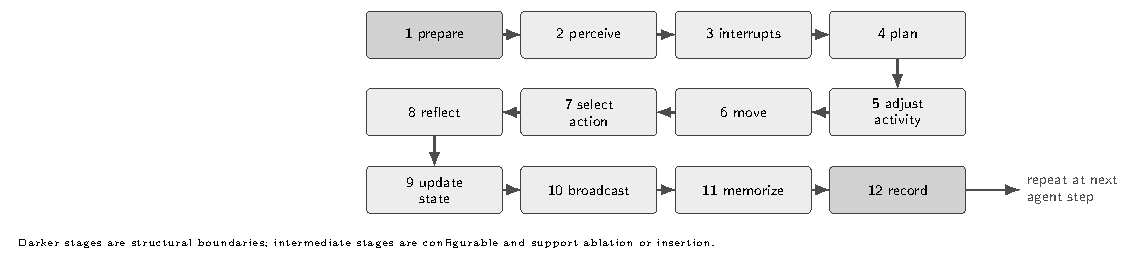
\includegraphics[width=\linewidth]{agent_lifecycle.pdf}
  \caption{The configured default agent-step pipeline.  The first and last
  stages are structural boundaries; intermediate stages may be omitted or
  replaced through configuration.  Domain inputs also arrive through direct
  calls, event-bus contribution points, plugin lifecycle hooks, and a player
  intervention queue; the diagram is a control-flow account rather than a
  claim that every subsystem is a plugin.}
  \label{fig:agent-lifecycle}
\end{figure}

\begin{figure}[t]
  \centering
  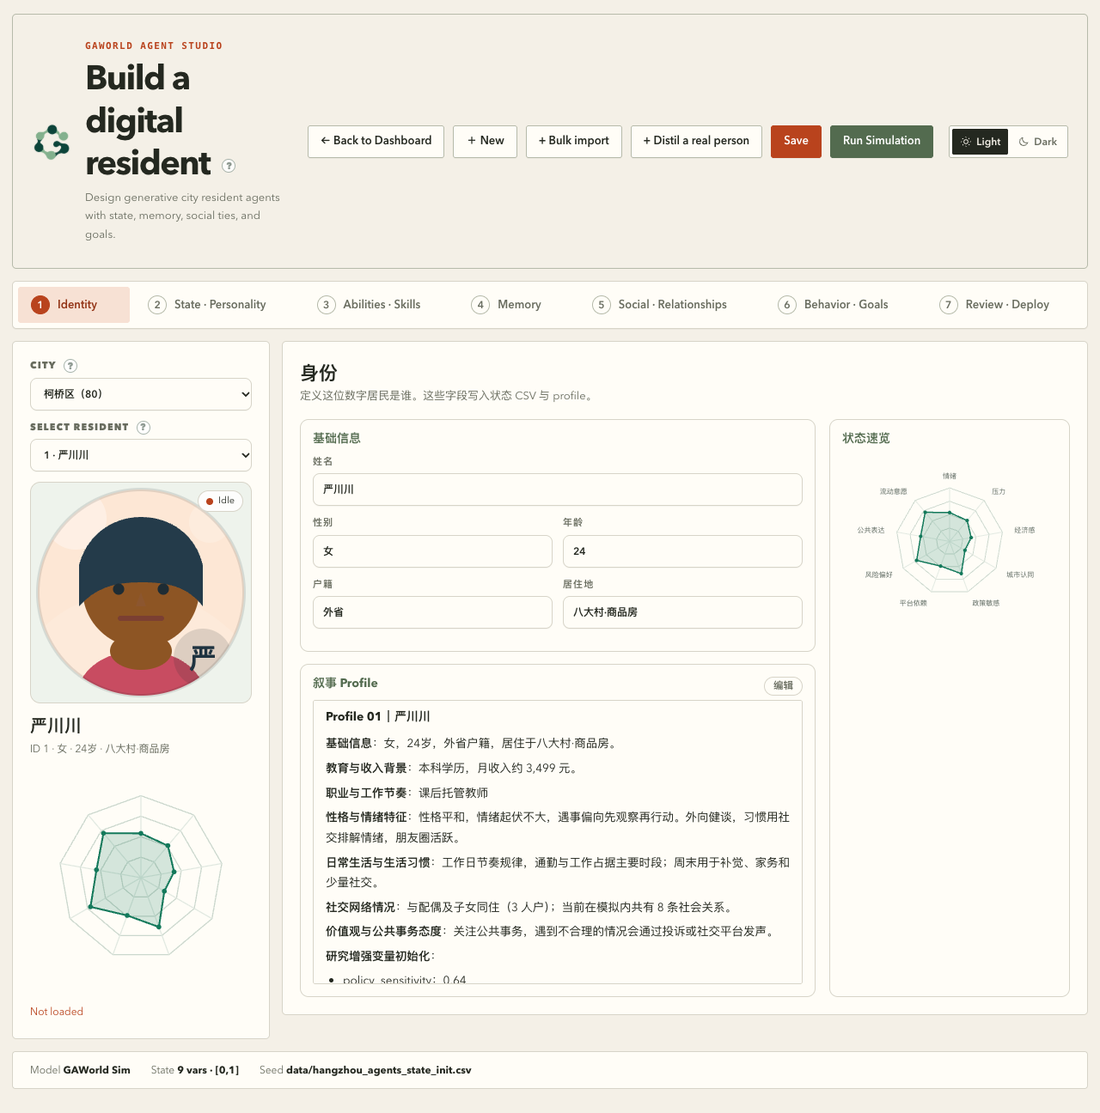
\includegraphics[width=\linewidth]{en_02_studio.png}
  \caption{The Agent Studio.  The seven-step tab at the top
  (\emph{Identity, State \& Personality, Abilities \& Skills, Memory,
  Social \& Relationships, Behavior \& Goals, Review \& Deploy}) maps one
  to one onto the seven sections of an Agent Studio session.  The left
  column selects the city and the resident; the right radar plots the
  normalized state across nine axes (activity, public-expression,
  pressure, economic sense, city recognition, policy sensitivity,
  risk preference, platform dependence, mobility intent).  The
  \emph{Profile} pane is the sourced-portrait view; the persona
  distillation module can write a similar portrait from a name or a
  URL through the \emph{Distill a real person} button on the top right.}
  \label{fig:agent-studio}
\end{figure}

\subsection{Profile seeds, mutable state, and personality}

At construction time, a tabular seed row supplies the identifier, demographic
fields, and initial scalar state, while a Markdown profile supplies descriptive
material such as occupation, daily life, and values.  The current builder
merges these sources into a dictionary containing \texttt{id}, profile fields,
\texttt{state}, an in-memory \texttt{memory} list, \texttt{social\_neighbors},
\texttt{personality} (Big-Five proxies), and \texttt{ext} (per-plugin
namespaces); it then initializes location against the city map and
personality against the configured personality plugin.  The core state includes
affective, socioeconomic, identity, behavioral, and information-exposure
variables.  Additional mechanisms may add namespaced or compatibility fields
during setup and execution.

v2 adds a \emph{personality plugin} that supplies Big-Five-derived proxies
(openness, conscientiousness, extraversion, agreeableness, neuroticism) for
every resident, used by the dynamic-interruption module and by selection
probabilities across the platform.  The plugin's anchors (a deterministic
fallback) and a model-derived overlay (an LLM cache keyed by a profile
signature) coexist; an experimental configuration can select the LLM overlay,
the deterministic anchors, or a custom provider.  The personality module also
maintains a corpus-rewrite pass that compares anchor distributions across
calibrators and warns when one trait dominates a group that the
configuration does not intend to dominate, in the spirit of recent work on
within-group flattening \citep{wang2025flatten}.

The class \texttt{gaworld.core.agent.Agent} is a typed adapter over the
backing dictionary.  It provides properties for identifier, name, state,
memory, schedule, location, attached skill identifiers, and personality
proxies, while dictionary access delegates to the same backing object.
\texttt{view\_as\_agent} therefore introduces no copy, and
\texttt{ensure\_agent\_dict} allows a typed caller to hand the record back to
older helpers.  This is important for incremental migration, but it is not a
fully typed agent schema: many runtime call sites still consume dictionaries,
and arbitrary mechanism-specific fields can still be added.

\subsection{Per-agent directory and persistence}

Persistence extends beyond the in-memory record.  Depending on enabled
features, per-agent directories hold episodic entries, diaries, schedules,
vector-indexed recall material, environmental preferences, private skills,
organization memberships, and travel itineraries.  On a stateful restart,
stored memory is loaded into the agent and can seed retrieval.  The file
boundary makes inputs to later decisions inspectable, although it also means
that reproducibility depends on capturing configuration, external model
behavior, and the complete artifact directory rather than only the seed CSV.

\subsection{The default per-tick path}
\label{sec:lifecycle:pipeline}

The cognition loop is implemented as an ordered \texttt{StagePipeline}.  A
stage receives an agent, a shared per-step dictionary, and the
\texttt{SimContext}.  Hook-visible values retain names such as
\texttt{activity}, \texttt{action}, \texttt{outcome}, and \texttt{reflection};
intermediate values use underscore-prefixed keys.  The default path contains
the following twelve stages, matching v1 with one explicit v2 addition:

\begin{enumerate}[leftmargin=*,label=\arabic*.]
  \item \textbf{prepare} establishes tick-local inputs and emits the pre-step
  boundary;
  \item \textbf{perceive} combines local environment, social, policy, memory,
  and contributed perception sections, including the indoor-room slot that
  names the room the agent is currently occupying;
  \item \textbf{interrupts} considers events that can alter the scheduled
  course, drawing on the dynamic-behavior module and personality proxies;
  \item \textbf{plan} forms the agent's immediate intention in the current
  context;
  \item \textbf{adjust\_activity} reconciles that plan with scheduled and
  interrupted activity;
  \item \textbf{move} resolves travel and updates location, then resolves the
  indoor room that the activity places the agent in (the v2 indoor-room
  hook fires here);
  \item \textbf{select\_action} chooses an action from the available action
  space, optionally mediated by a Controller validator chain;
  \item \textbf{reflect} produces an interpretation of action and outcome;
  \item \textbf{update\_state} applies state, relationship, and organization
  effects;
  \item \textbf{broadcast} exposes eligible communication to other agents or
  a distributed relay, including a player-say channel for human participants;
  \item \textbf{memorize} constructs and stores the tick's experience; and
  \item \textbf{record} appends established logs, state history, Recorder
  events, and visual trace material.
\end{enumerate}

Before the pipeline runs, the outer loop advances the shared Clock, updates
the environment and local occupancy, polls distributed messages when enabled,
and may perform configured information seeking.  After it returns, the
runtime emits \texttt{on\_agent\_post\_step}, allowing mechanisms such as the
intervention, governance, and organizations plugins to compute their own
metrics.  Day-start and day-end events bracket the tick loop; memory
consolidation, governance tallying, and organization-rule resolution are
invoked at the day boundary.  The twelve stages are therefore the agent-step
spine, not the entire simulation lifecycle.

\subsection{Contribution points and compatibility calls}

The EventBus lets a mechanism observe an event, contribute zero or more items,
or filter a value in priority order.  Perception composition is a concrete
example: local context can be assembled by established code while plugins add
bounded text sections without owning the full prompt.  Post-step and day-end
events similarly let policy, economy, skills, interests, organizations, or
governance react at defined boundaries.  Observer failures are logged and
isolated unless strict mode is enabled; stage failures instead propagate
because a missing control-flow stage could silently corrupt state.

Not all inputs use this bus.  Memory recall, environment evolution, and
social-network operations retain direct paths within or around the pipeline.
The Controller now validates structured movement requests and exposes audited
runtime interventions, but it does not mediate every selected action.
Likewise, \texttt{record} writes established artifacts in addition to the
kernel Recorder.  The lifecycle is connected and configurable while retaining
compatibility paths beyond the plugin boundary.

\subsection{Player interventions and the away state}

v2 adds two new first-class inputs to the lifecycle.  A \emph{player
intervention} arrives through the same Controller queue as scheduled events;
its type is one of \texttt{player\_claim}, \texttt{player\_act},
\texttt{player\_say}, or \texttt{player\_release}.  In a single-process
deployment, the intervention enters the local queue; in a multi-node
deployment, the hub routes the intervention to the node that owns the
resident, and the node enqueues it for the next tick.  Either way, the
intervention is then delivered to the agent's \texttt{interrupts} stage
(claim/release affect the lease) or \texttt{perceive} stage (act / say
appear in the next perception), and is recorded in the audit trail.  The
away state is a per-agent \texttt{travel} namespace that holds
\texttt{status}, \texttt{purpose}, \texttt{place}, \texttt{distance\_km},
\texttt{home\_node}, \texttt{depart\_day}, \texttt{return\_day}, and
\texttt{fare}; the agent's \texttt{locations.current} is rewritten to
\texttt{away (\textit{place})} so that occupancy calculations exclude the
agent without losing the round-trip.  Coming home restores
\texttt{locations.current} from \texttt{home\_node} so that travel time and
fare are computed against a real node rather than a label.

\subsection{Configuration and ablation semantics}

The stage order is read from \texttt{CONFIG["pipeline"]["agent\_step"]}.
Entries may name built-in stages or importable callables; a custom callable
can also receive a display name.  Unresolvable entries are skipped with a
warning, and an empty resolved pipeline is rejected.  Downstream built-ins
generally read absent step values defensively, which supports mechanism
ablations, but \texttt{prepare} and \texttt{record} are intended as
structural boundaries.  Changing order or removing a stage can change
semantics and artifact completeness.  The configuration surface enables
controlled system experiments; it does not guarantee that every permutation
is meaningful or behavior-preserving.

\section{Microkernel and Plugin System}
\label{sec:microkernel}

GAWorld v2 combines a connected cognition pipeline with a small kernel, a
registry of fourteen built-in plugins, and compatibility-preserving domain
paths.  The K1--K5 migration audited in v1 is now closed for the defined
scope, and a v2 audit covers three further migrations: \emph{multi-tenant
world resolution} (K6), \emph{distributed hub-and-node execution} (K7), and
\emph{parallel-worlds counterfactual execution} (K8).  The
\Cref{fig:system-architecture} freezes the v2 architecture at the audited
commit; existing capability cases are predate or postdate specific migrations
and are labeled accordingly in \cref{sec:capability-cases}.

\begin{figure}[t]
  \centering
  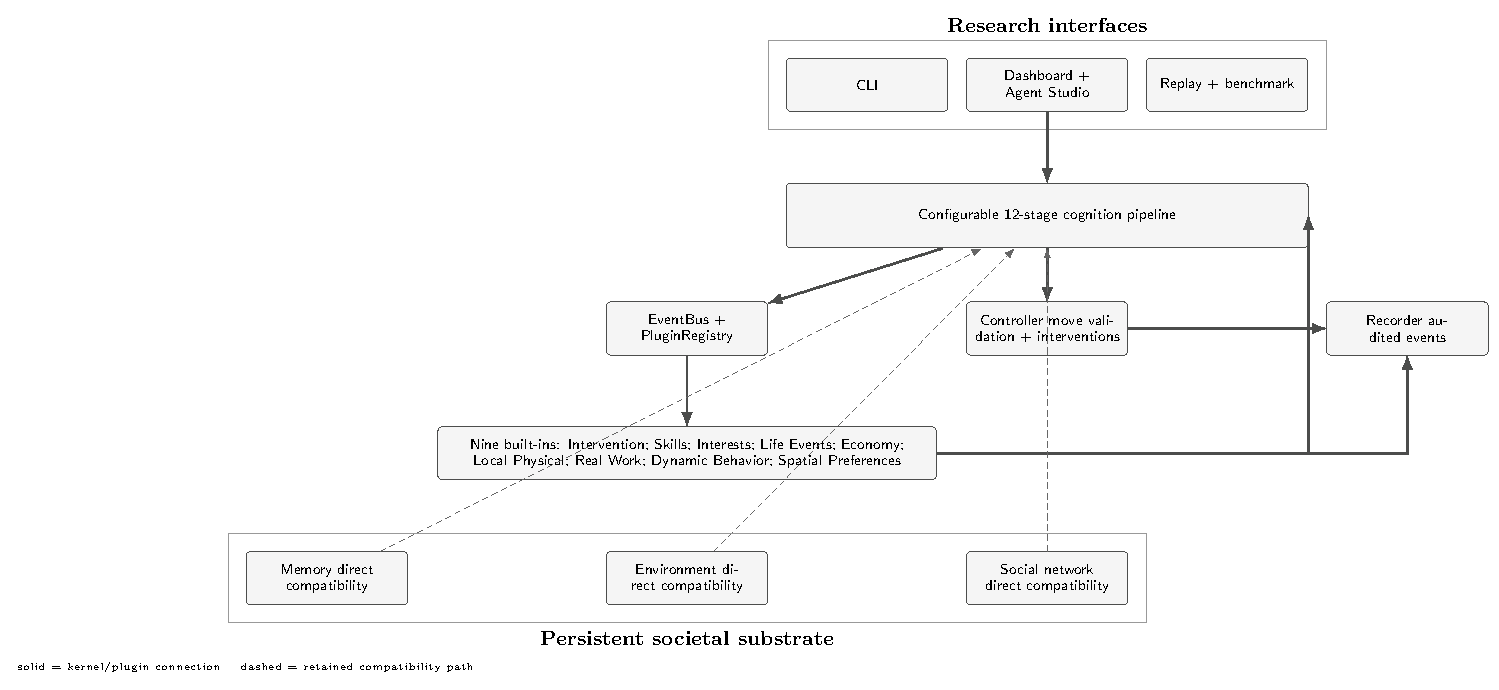
\includegraphics[width=\linewidth]{system_architecture.pdf}
  \caption{Audited v2 execution architecture.  The kernel (Clock, EventBus,
  PluginRegistry, Controller, Recorder, SimContext) serves the cognition
  pipeline and the per-tenant world resolver.  Fourteen built-ins contribute
  through the registry, bus, pipeline filters, or lifecycle events.
  Movement uses the Controller validation gate; Recorder events coexist with
  established domain-specific outputs.  In a multi-tenant deployment, the
  world resolver is the request-time entry point; in a multi-node deployment,
  the hub routes player interventions to the owning node.}
  \label{fig:system-architecture}
\end{figure}

\begin{figure}[t]
  \centering
  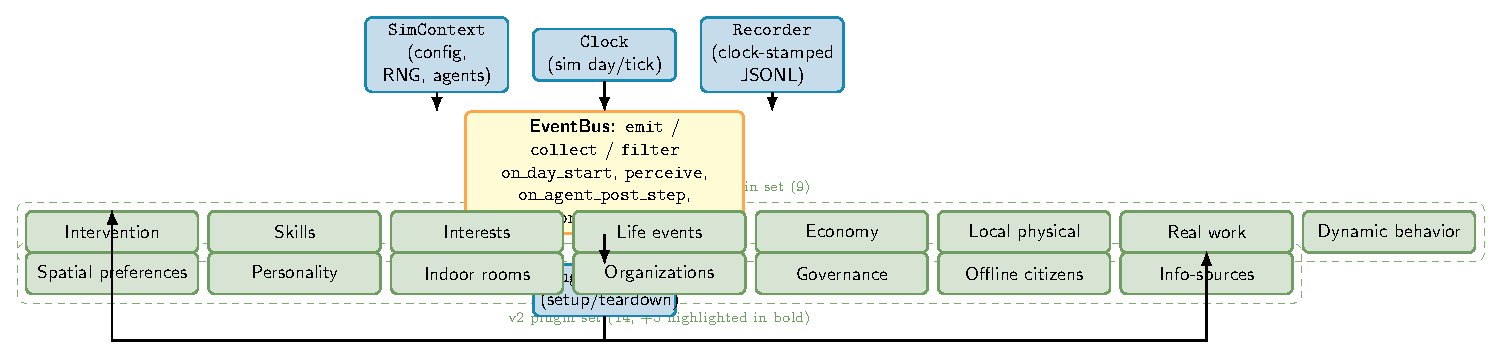
\includegraphics[width=\linewidth]{plugin_assembly.pdf}
  \caption{The fourteen v2 built-in plugins and their relationship to the
  kernel.  Plugins may subscribe to lifecycle events, contribute to
  perception, filter a value, or own namespaced state.  The v1 plugin set
  (nine) is shown above the v2 additions (five) for comparison.}
  \label{fig:plugin-assembly}
\end{figure}

\subsection{Kernel services}

\paragraph{Simulation context and clock.}
\texttt{SimContext} holds configuration, Clock, EventBus, PluginRegistry,
Controller, Recorder, agents and their identifier index, an LLM callable, a
seeded random-number generator, an \texttt{extras} compatibility escape
hatch, and (v2) a \texttt{WorldContext} reference to the active per-tenant
world.  It also provides simulation-level and per-agent plugin-state
namespaces.  The outer loop is the sole clock writer, giving stages, plugins,
and records a common simulated day, time, and tick.  This ordering does not
by itself make model calls, external services, or concurrency deterministic.

\paragraph{Event bus and plugin registry.}
The EventBus supports priority-ordered observation (\texttt{emit}), merged
contribution (\texttt{collect}), and value rewriting (\texttt{filter}).
Handler failures are logged and isolated by default, so warnings and active
plugin lists must accompany results.  The PluginRegistry assembles built-ins,
configuration-named classes, and installed entry points; orders setup by
declared dependencies; skips failed or unsatisfied plugins; and tears active
plugins down in reverse order.  Plugins may own configuration, namespaced
agent state, and output directories, but execute in process and are not a
sandbox.

\paragraph{Controller.}
The Controller provides a priority-ordered validator chain over structured
\texttt{ActionRequest}s and a named runtime-intervention API.  In the main
simulator, movement requests pass through validation: denial preserves the
origin and is surfaced in the next perception, while a rewrite can change the
destination.  The standard runtime interventions set one agent-state value,
update a dotted live-config path, queue agent removal for the next day
boundary, and (v2) deliver a player intervention to a specific node's queue.
Denials and interventions are audited through the Recorder.

\paragraph{Recorder.}
The Recorder appends clock-stamped JSON objects to table-specific files and
is closed when the simulation exits.  It records Controller activity,
distributed-hub activity, player interventions, and is available to plugins.
Main traces, state history, memories, environment events, and specialized
metrics also retain established writers.

\paragraph{World resolver (K6).}
The world resolver turns a request's authenticated user, a cookie indicating
the current world, and the caller's role into a \texttt{WorldContext} that
selects the active per-tenant configuration overlay, output root, run state,
and intervention queue.  Path-resolving functions in the dashboard and
simulation code consult the active world; module constants remain valid for
the \texttt{default} world so that single-tenant deployments and unit tests
behave identically.  When the account store is absent, the resolver
short-circuits to the \texttt{default} world.

\paragraph{Distributed hub (K7).}
The hub owns the per-world relay, the per-node intervention outbox, the
node-token store, and the global Recorder merge point.  The hub is the
\emph{dashboard server} when accounts are enabled and a thin
\texttt{cluster/hub} when accounts are not.  The hub does not advance
simulation time; it serves the run's record and routes messages.

\paragraph{Parallel-worlds engine (K8).}
The parallel-worlds engine runs up to eight matched worlds under a shared
seed and a per-world config patch, isolates each world's output tree, and
collects per-arm completion status and per-resident trajectory diffs for
post-hoc counterfactual inference.  It reuses the same event-bus,
Controller, and Recorder path; no domain code is changed between worlds.

\subsection{Built-in plugin assembly}

The audited registry assembles fourteen built-in plugins.  They attach
domain behavior to day/tick events, perception contributions, location
filters, action or outcome filters, and post-step or day-end hooks.  The
following table summarizes their declared surface and an indicative
per-agent or per-world state fragment.

\begin{table}[t]
\centering
\small
\setlength{\tabcolsep}{4pt}
\caption{The audited v2 plugin set.  Per-agent state column lists the
declarative fragment a researcher can read on a hashed run; the deployment
column lists the post-v1 changes each plugin enables.}
\label{tab:plugins}
\begin{tabular}{@{}p{0.20\linewidth}p{0.20\linewidth}p{0.18\linewidth}p{0.32\linewidth}@{}}
\toprule
Plugin & Lifecycle hook & Per-agent state fragment & v2 addition \\
\midrule
Intervention & on\_day\_start, post\_step & \texttt{ext.intervention} & cross-tenant metrics \\
Skills        & on\_agent\_post\_step, memorize & private skill library & skill consolidation by personality \\
Interests     & on\_day\_end, perceive & \texttt{ext.interests} & growth phase tracker \\
Life events   & on\_day\_start, on\_agent\_post\_step & \texttt{ext.life} & state effect normalization \\
Economy       & on\_day\_end, on\_agent\_post\_step & \texttt{state.econ} & endogenous inflation, credit-bound consumption \\
Local physical perception & perceive & local snapshot & indoor-room resolution \\
Real work     & on\_day\_start, on\_agent\_post\_step & \texttt{ext.work} & capability profile cache \\
Dynamic behavior & perceive, interrupts & \texttt{ext.dynamic} & personality-conditional interruption probability \\
Spatial preferences & filter (location) & \texttt{ext.spatial} & aversive-route rewrite \\
Personality   & agents.built, perceive & \texttt{personality} & Big-Five anchors + LLM overlay \\
Indoor rooms and venue capacity & agent.moved, perceive & \texttt{locations.room\_intent} & room-resolved occupancy and capacity \\
Organizations & on\_day\_start, on\_day\_end, on\_agent\_post\_step & \texttt{ext.org} & persistent org with role \\
Governance    & on\_day\_end, on\_day\_start & \texttt{ext.gov} & proposal/ballot engine \\
Offline citizens & agents.built & \texttt{ext.offline} & ghost taxonomy with visit / duty channel \\
\bottomrule
\end{tabular}
\end{table}

The adapters delegate calculations and specialized persistence to established
modules: migration changes orchestration and ownership, not the scientific
validity of the mechanisms.  The audit table in
\Cref{tab:migration-state} lists which subsystems have been fully
plugin-owned, which are partially integrated, and which retain direct
compatibility paths.

\subsection{Plugin authoring}
\label{sec:plugin-authoring}

A third-party plugin is a subclass of \texttt{gaworld.kernel.Plugin} with a
declared \texttt{id}, a tuple of plugin \texttt{requires} dependencies, a
\texttt{setup} method that receives \texttt{SimContext} and registers
\texttt{ctx.bus.on(...)} handlers, and a \texttt{teardown} method.  A plugin
can be installed by configuration, by entry point, or by code registration
\citep{gaworldplugin}.  Configuration and entry-point installation are
non-overlapping: a configured plugin runs even if it is not published as an
entry point.  Plugin setup failures are isolated: they produce a warning and
the affected plugin is deactivated, but the rest of the registry continues to
run.  This is intentional and is the reason the plugin set can be
reconfigured at runtime without an entire-process restart; it is also the
reason that an active plugin list, with its warnings, is part of every
research artifact.

\subsection{Migration-state audit}

\begin{table}[t]
\centering
\small
\setlength{\tabcolsep}{4pt}
\caption{Implementation state in the audited v2 repository.  ``Wired''
denotes a subsystem whose boundary is now the plugin surface; ``partial''
denotes an adapter that contributes but retains direct calls; ``retained
compatibility'' denotes a subsystem whose boundary is still the legacy
direct call.  K1--K5 cover the v1 migration; K6--K8 cover v2.}
\label{tab:migration-state}
\begin{tabular}{@{}p{0.20\linewidth}p{0.20\linewidth}p{0.18\linewidth}p{0.32\linewidth}@{}}
\toprule
Surface & Current boundary & Status (K) & Retained path and consequence \\
\midrule
Cognition & Configured 12-stage pipeline & Wired (K1) & Shared step dictionary; order and omissions must be reported \\
Extensions & EventBus and PluginRegistry & Wired (K1) & Failures may degrade rather than terminate a run \\
14 domain adapters & Policy, skills, interests, events, economy, physical, work, behavior, spatial, personality, rooms, organizations, governance, offline & Plugin-integrated (K1, K2) & Established stores and writers remain; activation needs config/plugin provenance \\
Memory & Recall, storage, consolidation, decay & Direct compatibility path (K3) & Persistent context is inspectable, not psychologically validated \\
Environment and social network & World evolution and network modules & Direct compatibility path (K3) & The full world and network models are not isolated plugins \\
Controller & Move validation, named interventions, player interventions & Connected, scoped (K4) & Other actions retain established paths; no universal-gate claim \\
Recorder & Clocked structured event writer & Connected, non-exclusive (K4) & Multiple writers remain; no single-log replay claim \\
World resolution & Cookie + account + role $\rightarrow$ WorldContext & Wired (K6) & When accounts are absent, single-tenant behaviour is preserved \\
Distributed hub & Per-world relay and per-node outbox & Wired (K7) & Best-effort delivery; no consensus, no clock synchronization \\
Parallel worlds & Up to 8 matched worlds, shared seed & Wired (K8) & Deterministic; no domain change between arms \\
\bottomrule
\end{tabular}
\end{table}

\subsection{Failure and reproducibility boundaries}

A cognition-stage exception propagates because the stage is control flow.
Bus-handler and plugin-setup failures instead warn and normally leave the
remaining run active; missing dependencies deactivate the affected plugin.
Operational resilience therefore makes a completed process different from a
complete treatment.  A reproducible artifact must include resolved stage
order, active plugin identifiers, warnings, configuration, source snapshot,
model/provider conditions, specialized outputs, the world identifier, the
node identifier (if any), and the player intervention trail (if any).  The
v1 description of K1--K5 remains accurate; v2 adds the requirement that the
artifact also record the world identifier, the node identifier, and the
per-arm completion status of every parallel-worlds study.  These additions
are not yet enforced by the kernel; the artifact ledger remains the
researcher's responsibility, with the schema documented in
\Cref{sec:validation-boundaries}.

\section{Memory, Cognition, and Behavioral Realism}
\label{sec:memory-cognition-realism}

v2 separates persistence from generation.  An agent's continuity is not held
solely in an LLM context window: structured state, episodic records, habits,
intentions, relationships, environmental preferences, growth profiles,
private skills, organizational membership, governance state, travel
itinerary, and personality proxies are written to mechanism-specific stores
and reintroduced at later steps.  Figure~\ref{fig:memory-growth} summarizes
this path.  The system can preserve and expose information across simulated
days; whether its memory dynamics resemble those of people is a separate
empirical question.

\begin{figure}[t]
  \centering
  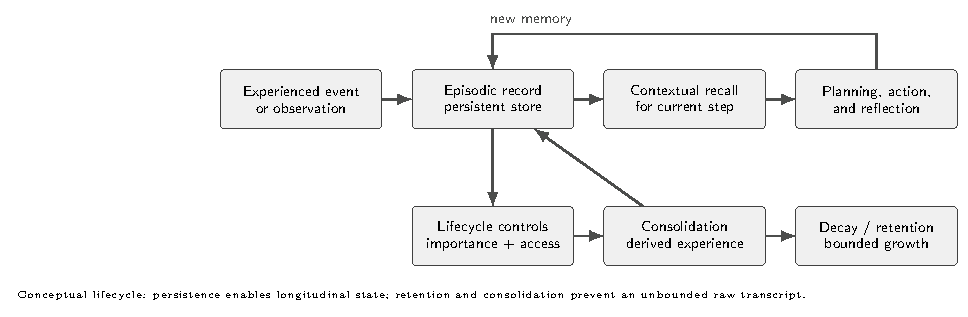
\includegraphics[width=0.94\linewidth]{memory_growth.pdf}
  \caption{Persistent experience and growth paths.  Tick-level episodes feed
  retrieval and rule-based updates; configured day-boundary processes may
  consolidate episodes into semantic memories or private skills, classify
  growth into a phase, drain the life-event queue, and tally governance
  ballots.  Solid storage paths denote implemented persistence, not validated
  models of human remembering or learning.  Dashed paths indicate optional
  LLM calls that may be disabled in a controlled experiment.}
  \label{fig:memory-growth}
\end{figure}

\subsection{Episodic persistence and retrieval}

The basic store retains an agent's memory list, schedule, available actions,
locations, and location--action biases as JSON, alongside append-only textual
logs and simulation state.  A second experience layer records episodes in
JSONL and persists habits, daily intentions, relationships, and environmental
preferences in separate per-agent files.  This division supports inspection
and selective restart, although a complete restart requires all of these
stores rather than a single canonical agent file.

For content-addressed recall, memory entries are also indexed in SQLite with
type, simulated time, salience, recall count, and an embedding.  The
configured embedding path may call an embedding provider; if that path is
unavailable, the implementation falls back to a deterministic hash embedding.
Retrieval combines vector similarity with salience, age decay, and prior
recall, then optionally boosts entries related to the agent's current growth
interests.  Thus ranking is a specified scoring procedure over stored entries,
whereas the text being ranked may have originated in an LLM-generated action,
reflection, diary, news item, or external source.

The day-boundary lifecycle adds two optional transformations.  Consolidation
selects recent episodic rows and asks an LLM to distill them into a small set
of semantic entries; malformed output or insufficient material produces no
new entry.  Decay is LLM-free: after a configured period it lowers the
salience of old, unrecalled episodic rows and deletes rows already below a
floor, while protecting semantic, external-information, and procedural
entries.  A separate episode store also computes exponential salience decay
and enforces a size cap.  These two decay paths operate over different stores
and should not be mistaken for one unified cognitive theory.

External retrieval-augmented memory is also optional.  v2 unifies three
external-memory paths behind a single \texttt{info-sources} surface: a
keyword-driven web-search RAG \citep{gaworldrag}, an agent-derived query
flow that retrieves web material, and a configured \emph{information diet}
that mixes social, news, and professional sources per agent.  After retrieval
an LLM may assess or compress the material into external-information
entries.  This path depends on a caller-supplied fetch adapter and degrades
to no operation on failure.  Consequently, an experimental report must
disclose whether external retrieval, provider-based embeddings,
consolidation, and decay were enabled.

\subsection{Intentions, habits, and reactive behavior}

Behavioral continuity combines model-mediated interpretation with explicit
state-transition rules.  At day boundaries, recent episodes and current state
can be supplied to an LLM to produce priorities, avoidances, social targets,
and recovery goals.  When the call budget is exhausted or parsing fails, a
rule-based fallback constructs intentions from state and recent experience.
Habit strength, relationship signals, physiological and time-pressure needs,
episode salience, and many mood or stress adjustments are updated by bounded
numeric rules.  These values enter subsequent prompt context rather than
being left as unstructured prose.

The dynamic-behavior module evaluates candidate interruptions from needs,
co-location, incoming messages, environmental events, local physical
conditions, cascades, and spontaneous urges.  Acceptance probabilities
depend on event intensity, activity commitment, personality proxies,
relationship closeness, and agent state.  Candidate generation and schedule
insertion are LLM-free but stochastic; they are repeatable only when the
relevant random state is seeded.  Once an interruption wins, the ordinary
activity-adjustment or action path may invoke an LLM to phrase or refine the
response.  v2 therefore distinguishes rule-based opportunity and constraint
generation from model-generated interpretation and action text, and adds a
\emph{personality-conditional} acceptance probability drawn from the Big-Five
proxies the personality plugin supplies.  The configuration can disable this
overwrite and recover the v1 behavior; the artifact ledger records which
version was active.

Spatial preference illustrates continuity without language generation.  A
crowd surge or other location anomaly raises a time-bucketed aversion score;
scores decay with recency, and a later destination can be redirected when its
aversion crosses a configured threshold.  This mechanism implements learned
avoidance as a transparent rule.  It does not establish that the learning
rate, threshold, or decay reproduces human spatial choice.

\subsection{Interests, skills, and productive activity}

Growth profiles contain bounded hobby and skill items with phase, engagement,
competence, practice history, and activity templates.  Their initial content
may be derived by an LLM and cached by a profile signature; deterministic
fallback profiles are available when generation fails.  Episode matching,
practice updates, phase classification, daily retention decay, retirement of
stale interests, and socially mediated adoption then use explicit rules and a
seedable random generator.  The labels borrow a developmental vocabulary, but
their implementation is a simulation mechanism rather than a validated model
of human interest development.

The skill subsystem maintains a curated global library and per-agent private
skills.  Available skills can be injected into cognition context, while an
optional LLM consolidation step extracts a reusable procedure from recent
episodes and saves it as a private Markdown skill.  Parsing, schema checks,
and registry precedence constrain this output; they do not demonstrate that
the procedure is correct or transferable outside the generated setting.

Productive activity extends this pattern to a mock work market.  Cached,
LLM-derived capability profiles and current growth items inform routing.  A
JSONL queue provides claim and recovery semantics, a worker pool dispatches
briefs concurrently, and code, content, teaching, and web-design adapters use
an LLM to produce files.  Lightweight validators check properties such as
Python syntax, Markdown structure, or HTML/SVG parseability before successful
results are ingested into agent state and market settlement.  These checks and
persisted artifact paths demonstrate a functioning production pipeline; they
are not evidence that an artifact meets professional, pedagogical, factual, or
security standards.

\subsection{Realism module and personality anchoring}
\label{sec:memory:realism}

v2 exposes a \emph{realism module} (\texttt{gaworld/cognition/realism.py})
that contains the heuristics used to make generated text more human-like
without claiming a psychological theory.  Concrete entries include
non-clich\'e opening moves, time-of-day salutations, the calibration of
mood to the day's events, and the suppression of repeated openings in
successive diary entries.  The realism module is consulted through
\texttt{on\_day\_start} and \texttt{on\_agent\_post\_step}; a configuration
can disable it for a baseline run.  v2 also adds a personality-anchor
\emph{rewriter} that, when invoked with an LLM overlay, calibrates Big-Five
proxies against a corpus and warns when one trait dominates a group that the
configuration does not intend to dominate.  The rewriter is opt-in, and the
artifacts that opt in record the calibration set, the resulting
distributions, and a SHA-256 hash.  The rewriter does not establish
psychological validity; it is a controlled, inspectable mitigation of
flattening, not a substitute for a held-out evaluation.

\section{Situated Urban and Societal Substrate}
\label{sec:substrate}

GAWorld v2 places persistent agents in a shared substrate whose components
read and write overlapping state.  The city constrains movement, the indoor
spatial tree constrains co-location, local occupancy changes perception,
relationships affect encounters, financial or life events alter later
choices, organizations impose rules, governance proposes and votes on rule
changes, and information exposure shapes what residents believe.  This
coupling supports questions that cross individual and aggregate levels, but
it also means that mechanism provenance and configuration are part of every
experimental treatment.

\subsection{City graph and indoor spatial tree}

The city map parses places, roads, transit lines, interiors, and land-use
attributes into a graph.  Nodes carry categories, coordinates, capacity,
opening hours, popularity, density, and display metadata.  Destination
resolution can match activity terms to place categories, while graph routing
and transport-mode rules estimate distance, time, and fare.  Mode speeds,
fixed delays, road-class multipliers, rush-hour penalties, area price levels,
and weather preferences are explicit parameters.  They make travel costs
inspectable; their presence does not imply transport-model calibration.

v2 extends the city graph with an \emph{indoor spatial tree} that resolves
every indoor activity to a specific room in a building.  The tree shares its
layout vocabulary with the front-end visualizer, so that back-end simulation
and front-end display agree on which room an agent is in.  Eighteen layouts
(residential, apartment, hotel, hospital, clinic, pharmacy, school, library,
shop, cafe, restaurant, office, government, factory, station, gym, park, and
public space) map activity terms to furniture slots (sleep, cook, exercise,
\ldots).  When the spatial-tree plugin is enabled, indoor co-location
restricts a meeting to the same household and the same room; venue capacity
is per-room, computed as a fraction of the venue's capacity that the room
occupies in its layout.  When the plugin is disabled, the v1 behavior is
preserved.

At each tick, the local-physical layer recomputes occupancy from stationary
agents, clears stale counts, and exposes the current location's crowding,
opening status, and weather.  A crowd anomaly is flagged when occupancy is
both high and sharply above the previous tick.  These snapshots can enter
perception and interruption generation, linking collective movement to
individual behavior.  The mechanism is deterministic given agent locations
and parameters, although the locations themselves may follow stochastic or
LLM-mediated decisions.

\subsection{Environment, weather, and crowd anomalies}

The broader environment system supports configured natural, economic,
political, technological, and intraday events.  In rule mode it samples from
configured event distributions using a local random generator.  In LLM mode
a model proposes a daily summary, events, and intraday rules that are
parsed into the same bounded event schema; configured fallback generation
remains available if that call fails.  Severity and anomaly tagging are
rule-based.  v2 separates \emph{natural} events (weather, accident,
epidemic) from \emph{social} events (rumor, market shock, policy reform) and
exposes a \emph{crowd anomaly} channel that the local-physical layer writes
into a single perception field.  Reports must therefore identify the
generator mode rather than treating all environmental histories as
equivalent.

\subsection{Social ties, life events, and offline citizens}

Relationships are typed records rather than undifferentiated neighbor edges.
Role templates specify channels, obligation, protection, and daily decay;
interaction signals update closeness and contact time.  The implementation
can bootstrap off-screen contacts from an LLM-generated backstory, with a
deterministic heuristic fallback.  v2 adds an \emph{offline citizen}
subsystem that classifies each ghost contact by relationship role and
admission channel (call, message, visit, none), produces stateful obligations
when a contact is long-neglected, and exposes a visit channel that the
\emph{travel} plugin \citep{gaworldtravel} actually exercises.  The combined
offline + travel stack turns a previously read-only field (the obligation
counter) into a behaviorally consequential signal.

Maintenance is rule-based.  Uncontacted ties decay at role-specific rates,
long-neglected obligations can rise, and an enforcement pass assigns nested
Dunbar-style tiers while pruning beyond a configured outer cap and protecting
selected kin roles.  These tiers are an operational capacity constraint, not
evidence that the simulated network reproduces measured human networks.

Life events are normalized, persisted, scheduled by simulated day and time,
and drained once when due.  Events can target agents and carry bounded state
effects and tags.  v2 makes life-event state effects typed and reversible:
each effect has an effect-id, a magnitude, a half-life, and a reversal hook,
so a cancelled event can be undone at the day boundary without leaving
free-floating state.  This is a controlled exogenous-event surface whose
timing and direct updates are inspectable; the realism of event frequencies,
dependencies, and consequences must be established by a separate study.

\subsection{Economy, credit, and endogenous inflation}

The finance module maintains checking, savings, investment, and housing-fund
accounts; monthly budgets; income and expense records; liabilities and
credit; sector pools; government flows; and macro state.  Configured rules
calculate social-insurance deductions and progressive income tax, route wages
and consumption, enforce available-cash and credit constraints, transfer
savings, and settle payments.  A dedicated seeded random generator drives
expenditure variation, market returns, shocks, and other probabilistic
transitions so that unrelated random draws need not perturb the economy
sequence.

v2 closes a long-standing gap: the v1 code reported an inflation rate and a
price index that no other component read.  In v2 the price level multiplies
real expenditure so that wages that do not follow it produce a measurable
erosion of real consumption.  Inflation itself is endogenized through a
\emph{demand-pull} rule: $\pi = \pi^{*} + \kappa \cdot (C/C_0 - 1)$, where
$C$ is a 30-day moving average of real per-capita consumption, $C_0$ is the
first 30 days as a baseline, and $\pi$ is clamped to a configured interval
\citep{gaworldinflation}.  The wage index, when enabled, ties a fraction of
new wages to the price level.  This is the first run at making
``cost-of-living erosion'' actually measurable in a GAWorld run, and the
artifact ledger records whether the wage index was active so that the
directional claim is not silently over-interpreted.

Shared sector and government pools make counterparties visible instead of
creating every monetary flow without an account.  Agent-to-agent payments
and some rent or labor flows can be routed to modeled recipients;
investment returns combine a common market component with idiosyncratic
variation.  Ledger and conservation checks can reveal implementation defects
such as unbalanced internal transfers.  They cannot establish that the tax
schedule, consumption response, labor process, credit behavior, or macro
dynamics is an empirically valid representation of a real economy.
Accounting consistency is therefore a software invariant, not a
behavioral-validation result.

\subsection{Organizations, governance, and rule changes}

v2 adds a persistent-organization subsystem.  Each organization is a
typed object (community, business, club) with members, role templates, a
chosen governance mode (\emph{off}, \emph{leader}, \emph{member-vote}), and
a ruleset that the plugin applies on member decisions.  Two rule-change
pipelines exist: a \emph{leader} pipeline in which a designated member
decides, and a \emph{member-vote} pipeline in which a proposal is opened,
voted on, and (if it passes) enqueued for application at the next day
boundary \citep{gaworldgovernance}.  Generations are isolated: a proposal
opened under a given member snapshot, governance version, and ruleset cannot
be re-opened after the world is rebuilt with a different member snapshot.
This isolation is enforced in a single SQLite transaction.

The governance subsystem is opt-in (\texttt{governance.enabled}); when it is
off, the v1 organization behavior is preserved.  Vote tallies and rule
versions are recorded in a separate \texttt{governance.json} per generation,
not interleaved with the per-step metrics CSVs, so that governance results
do not contaminate aggregate economic measurements.

\subsection{Information sources and Moltbook}

v2 unifies information exposure under an \emph{info-sources} surface
\citep{gaworldrag}.  Each resident has a configured diet (a list of
channels and a sampling rate) and a per-tick search budget.  Channels cover
local news, social posts, professional feeds, and (when enabled) web
search.  The Moltbook integration gives residents a social network identity
(\texttt{gaworld/moltbook}) where they post, reply, and react; the agent's
actions in Moltbook are recorded as separate \texttt{log.jsonl} entries,
distinct from simulation traces, and are summarized back into the perception
field at the next tick.  This separation lets a researcher inspect the
social-network behavior of a resident without conflating it with the
simulation's per-step state history.

\subsection{Coupling and ownership boundaries}

\Cref{tab:component-coupling} makes the principal shared-state paths
explicit.  ``Implemented'' refers to an inspectable current mechanism;
``partial boundary'' indicates that the mechanism is connected but retains
direct calls, shared dictionaries, or specialized writers rather than a
fully isolated plugin interface.

\begin{table}[t]
\centering
\small
\setlength{\tabcolsep}{3.5pt}
\caption{Coupling among agent and societal components.  Evidence status
describes implementation visibility, not empirical validity.}
\label{tab:component-coupling}
\begin{tabular}{@{}p{0.13\linewidth}p{0.16\linewidth}p{0.16\linewidth}p{0.27\linewidth}p{0.16\linewidth}@{}}
\toprule
Subsystem & Reads & Writes & Agent-visible consequence & Evidence status \\
\midrule
Memory and cognition & Episodes, state, context, retrieved entries & Memories, intentions, habits, relationships & Recalled context, priorities, reflection, later action bias & Implemented; human realism unvalidated \\
Interests and skills & Profile, episodes, social growth context & Growth profile, private skills & Practice focus and procedural prompt context & Implemented; partial plugin boundary \\
World and local physics & City graph, time, weather, locations, rooms & Routes, travel state, occupancy snapshots, room occupancy & Feasible destinations, travel costs, crowding, closure cues, room-level co-location & Implemented; direct integration \\
Environment & Configuration, history, optional LLM output & Events, weather and macro context & Interruptions and perceived exogenous conditions & Implemented; generator-mode dependent \\
Social network & Profiles, contact history, interactions & Typed ties, closeness, obligation, tiers & Encounter probability and relationship context & Implemented; mechanism validity unassessed \\
Life events & Persisted event queue, clock & Consumption flag and configured state effects (typed, reversible) & Scheduled exogenous changes to targeted agents & Implemented; committed plugin-integrated event producer \\
Economy & Activity, balances, calendar, sectors, macro state, price level & Accounts, ledger, budgets, pools, agent state, end-of-month price index & Income, spending constraints, taxes, credit, returns, payments, real-consumption erosion & Implemented; primarily hook-based \\
Work & Capability cache, activity, growth, market jobs & Queue results, artifacts, settlement and state effects & Produced files, earnings, experience records & Implemented; artifact quality unvalidated \\
Indoor rooms and capacity & City map, location, activity & Per-room occupancy, capacity enforcement, room-intent binding & Room-resolved perception, capacity-based rejection & Implemented; opt-in \\
Personality & Profile, optional LLM overlay & Personality proxies & Conditional interruption probability, growth-phase weighting & Implemented; anchor + overlay \\
Organizations and governance & Membership, role, ruleset, proposal & Updated ruleset, accepted proposal, vote tallies & Rule-conformant behavior, post-vote transitions & Implemented; opt-in \\
Offline citizens and travel & Off-screen contact roles, duty obligations & Visit channel, trip itinerary, location rewrite & Mobile-agent perception, family duty fulfillment & Implemented; opt-in \\
Information sources & Channel list, search budget, agent-derived query & Retrieved entries, Moltbook posts, perception field & Exposure heterogeneity, search-induced awareness & Implemented; channel-dependent \\
\bottomrule
\end{tabular}
\end{table}

The table exposes the current modularity limit.  The 14 built-in plugins
have plugin entry points; economy, local physical perception, spatial
preferences, work, dynamic behavior, indoor rooms, organizations,
governance, personality, offline citizens, and information sources have
built-in adapters.  Memory, environment evolution, and social-network
operations still exchange mutable agent dictionaries or runtime objects
directly.  This arrangement is usable and inspectable, yet replacing one
mechanism can change prompts, state schemas, random draws, and specialized
artifacts elsewhere.  Controlled comparisons should therefore freeze the
complete coupled configuration rather than naming only the focal
intervention.

\section{Multi-User, Multi-World, and Per-Tenant Isolation}
\label{sec:multi-user-worlds}

GAWorld v2 makes a \emph{World} a first-class object.  A world is a city
bundle plus a per-world configuration overlay plus a per-world output root
plus a per-world set of memberships.  The active world is resolved from a
cookie, validated against the caller's role, and propagated through a
context variable.  This section describes the data model, the
request-resolution path, the run-management machinery, the visibility
rules, the static-file guard, and the per-tenant quotas.  When the account
store is absent, the single \texttt{default} world is the only world, and
the system behaves as it did before multi-tenancy was added.

\begin{figure}[t]
  \centering
  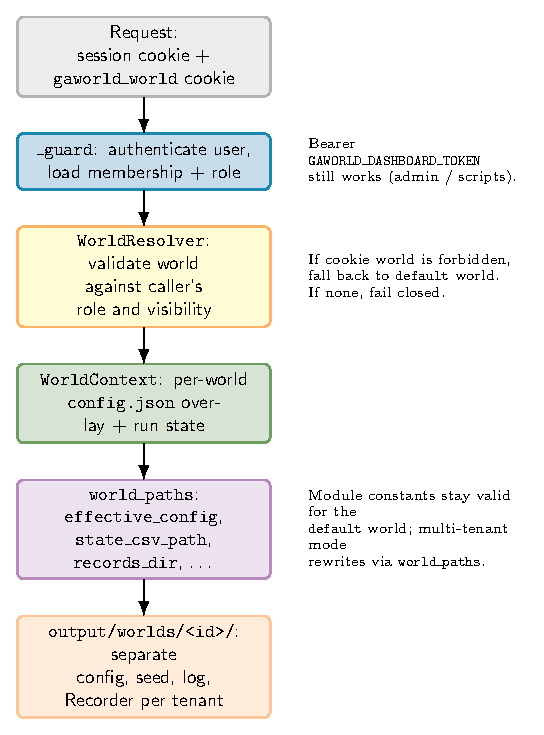
\includegraphics[width=\linewidth]{multi_tenant.pdf}
  \caption{Request resolution in a multi-tenant deployment.  A request enters
  the dashboard server with a session cookie and a \texttt{gaworld\_world}
  cookie; \texttt{\_guard} authenticates the caller, the \texttt{WorldResolver}
  validates the cookie against the caller's role and visibility, and the
  resulting \texttt{WorldContext} drives per-tenant path resolution.}
  \label{fig:multi-tenant}
\end{figure}

\begin{figure}[t]
  \centering
  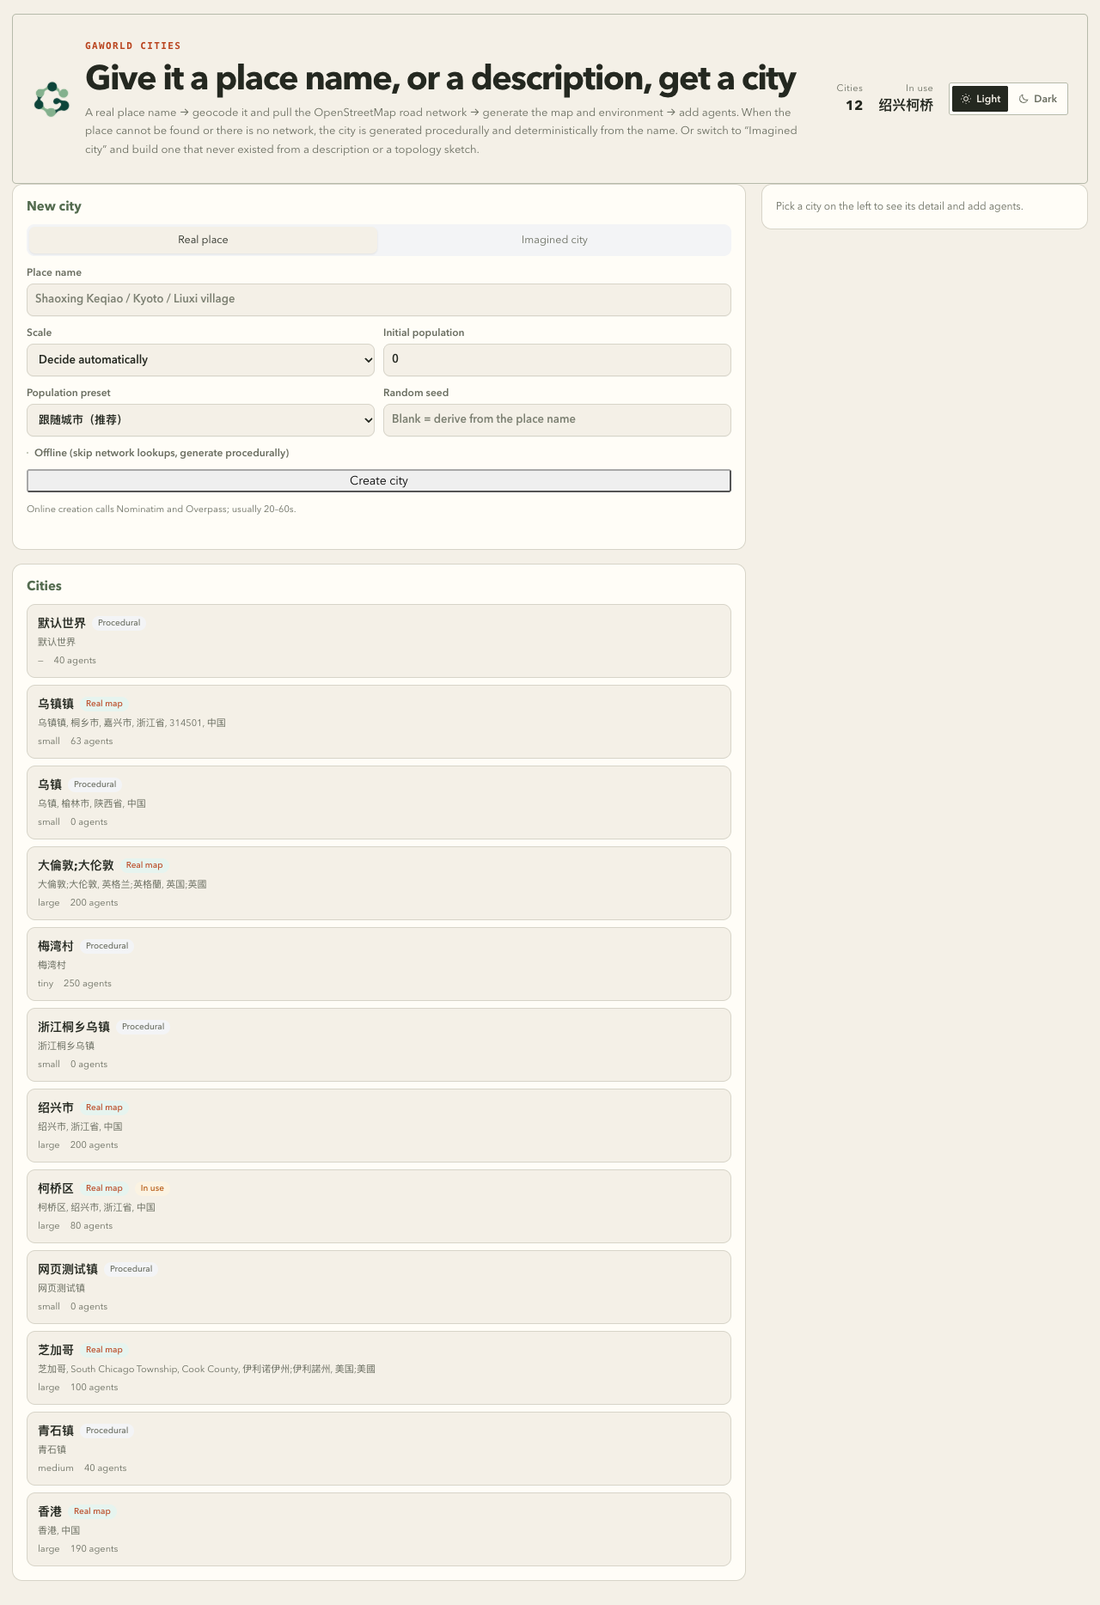
\includegraphics[width=\linewidth]{en_07_citymap.png}
  \caption{The Cities panel.  A v2 deployment lists every city bundle it has
  access to; the panel creates a new city from a real place name (geocoded
  via Nominatim with OpenStreetMap data) or from an imagined description
  (procedurally generated).  Each entry shows the source (\emph{Real map} or
  \emph{Procedural}), the scale (\emph{tiny / small / medium / large}), and
  the agent count.  Selecting a city loads its bundle into the running
  world; the \emph{In use} tag indicates the bundle currently driving the
  active simulation.  This panel is the entry point for per-tenant world
  isolation: when accounts are enabled, each user has a personal \emph{In
  use} pointer and a list of worlds they own or can join.}
  \label{fig:cities}
\end{figure}

\subsection{Data model}

A v2 deployment, when accounts are enabled, stores the following objects in
an SQLite database (\texttt{output/accounts/accounts.sqlite}, no new
dependency):

\begin{itemize}[leftmargin=*]
  \item \textbf{User} with one of two roles: \emph{admin} (teacher) or
  \emph{member} (student), and an optional capability bit
  \texttt{can\_create\_city};
  \item \textbf{Session} storing only a SHA-256 hash of a 32-byte random
  token, with \texttt{HttpOnly; SameSite=Strict} cookies;
  \item \textbf{Invite} generated in batches, optionally labelled, with an
  expiry and a quota template;
  \item \textbf{World} referencing a city bundle, a per-world configuration
  file, and a visibility level;
  \item \textbf{Membership} binding a user to a world as
  \emph{owner}/\emph{player}/\emph{observer};
  \item \textbf{Usage} and \textbf{audit} records for per-tenant quotas and
  forensic replay.
\end{itemize}

A world is a folder under \texttt{output/worlds/\textit{world\_id}/} that
holds the city's \texttt{agents.csv} and \texttt{profiles.md} as
copy-on-write \texttt{seed/} files, the run log, the run-time
configuration overlay, the run state, the intervention queue, and the
Recorder.  When the world is deleted, the folder is removed; when the user
account is deleted, every owned world is deleted with it.  A world is also
the natural unit of distributed execution (see
\Cref{sec:distributed-playable}).

\subsection{Request resolution}

A request enters the dashboard server with a session cookie, a
\texttt{gaworld\_world} cookie indicating the caller's chosen world, and
(optionally) a Bearer token.  The \texttt{\_guard} middleware authenticates
the caller and loads the membership.  The world resolver then:

\begin{enumerate}[leftmargin=*,label=\arabic*.]
  \item reads the caller's \texttt{gaworld\_world} cookie;
  \item verifies that the world exists and that the caller has at least
  \emph{observer} visibility;
  \item if not, falls back to the shared \texttt{default} world (a
  per-tenant deployment may have no such world, in which case the request
  fails closed);
  \item loads the world's \texttt{config.json} and merges it with the global
  \texttt{dashboard\_config.json} under a documented precedence order;
  \item sets a \texttt{ContextVar} that downstream code consults in lieu of
  reading global configuration; and
  \item selects a path-resolving function for the world's output root.
\end{enumerate}

This pattern preserves all module-level path constants in the v1 code:
\texttt{output/} is still the default world's root, and the same code that
reads a relative path in a single-tenant deployment reads a world-rooted
path in a multi-tenant deployment.  Unit tests that monkey-patch module
constants continue to work; the dashboard does not require a new fork
because of multi-tenancy.  A pitfall identified during the migration is
that \texttt{python -m gaworld.apps.dashboard\_server} previously loaded
the module a second time as \texttt{\_\_main\_\_}, producing two parallel
world resolvers.  The fix was to delegate the \texttt{-m} entry point to
the canonical module and to add a regression test
(\texttt{ModuleEntryPointTest}).

\subsection{Path resolution and output isolation}

Without multi-tenancy, the simulation wrote to a fixed set of paths under
\texttt{output/}.  v2 adds a path-resolution layer (\texttt{world\_paths})
that takes a base root and returns the per-world versions of each path.
The base layer is unchanged for the default world, so single-tenant
deployments see no behavior change.  For a multi-tenant deployment, the
path layer reads \texttt{effective\_config} and \texttt{world\_root} from
the context variable and rewrites the \texttt{RUN\_PATHS} entries
(\texttt{memory\_dir}, \texttt{state\_output\_dir}, and
\texttt{kernel.interventions\_path} for the simulation, plus
\texttt{records.output\_dir} and \texttt{records.interventions\_path} for
the dashboard) to the world's root.

A run is launched in the world's process group with
\texttt{GAWORLD\_CONFIG\_OVERRIDES} carrying the world-specific paths.  The
simulation code does not need to know which world it is in; it reads the
override environment variable and writes to the resolved paths.
A configuration change in a world's \texttt{config.json} therefore takes
effect at the next run boundary without restarting the dashboard.

\subsection{Visibility and roles}

A world's visibility is one of \emph{private}, \emph{class}, or
\emph{open}.  A \emph{private} world is visible only to its owner (and any
admin).  A \emph{class} world is read-only for all members; teachers use it
to publish a demonstration world.  An \emph{open} world allows any member
to join; joining creates a \emph{player} membership that lets them claim
residents and act in the simulation.  A \emph{player} can also be downgraded
to an \emph{observer}; an \emph{observer} can read state, profiles, and
memory but cannot mutate anything.

Roles are enforced at the API layer, not at the run layer: the run itself
is unaware of who is watching, but a write to the world is checked against
the caller's role before being applied.  This is the same trust model as
the v1 system but with a finer-grained permission set.

\subsection{Run management and quotas}

A world can have at most one running simulation at a time; the dashboard
also enforces two global limits configurable by the admin:

\begin{itemize}[leftmargin=*]
  \item \texttt{max\_concurrent\_runs} (default 4): the maximum number of
  simulations across all worlds in the deployment;
  \item \texttt{max\_runs\_per\_user} (default 1): the maximum number of
  concurrent simulations per user (admins are exempt).
\end{itemize}

A run request that exceeds a limit is enqueued in a FIFO queue whose head
is the run with the earliest request time; the dashboard reports
``queued (position $k$)'' in the panel.  A user can withdraw a queued
request without affecting other users.  Quotas and queue state persist
across dashboard restarts.

\subsection{Static-file guard}

v2 introduces a static-file guard that requires an authenticated session
cookie to read any path under \texttt{output/} or \texttt{data/}.  The v1
implementation had only a single-token guard and rejected paths whose
basename began with a dot; this was insufficient because a logged-in user
could read other worlds' output.  The v2 guard checks the world
identifier, the caller's role, and the path's owner world before
returning the file.  Static assets outside \texttt{output/} and
\texttt{data/} (CSS, JS, fonts, HTML) are unaffected.

\subsection{Per-tenant ledger and audit}

Every mutation that crosses the API is recorded in the \texttt{audit}
table, with the caller's user id, the world's id, the operation type, the
target entity, and a timestamp.  The audit table is small (one row per
write) and is intended for forensic replay rather than as a primary
trace.  A per-tenant \texttt{usage} table records the number of LLM calls
the tenant has made, broken down by model, by task, and by day.  The
quota system reads from \texttt{usage} and refuses to start a run that
would push the tenant over the daily quota; a configurable dry-run mode
warns without refusing.

\subsection{Backwards compatibility and migration}

The migration to v2 is, by design, backwards compatible.  The
\texttt{AccountStore} is optional: an installation that does not run
\texttt{python -m gaworld.accounts init} continues to behave exactly as
v1 did, with \texttt{GAWORLD\_DASHBOARD\_TOKEN} as the only credential.
A first admin can be created with the same command; from that point on,
\texttt{\_guard} requires a session cookie or a Bearer token, and
\texttt{GAWORLD\_DASHBOARD\_TOKEN} is reserved for scripts and
back-compat.  A migration script exists for installations that want to
adopt multi-tenancy without re-creating their world, but most production
deployments start fresh.  This is the only way to preserve the byte-for-byte
single-tenant behavior that v1 promises; v2's promise is that single-tenant
behavior is preserved exactly when the account store is absent.

\section{Distributed Worlds and Playable Cities}
\label{sec:distributed-playable}

v2 introduces a hub-and-node protocol that lets a single open world be
partitioned across many machines.  The hub is the dashboard server; each
node is a worker machine that runs the simulation for a subset of the
world's residents with the node's own model key.  Players continue to
interact through a browser; the hub routes their interventions to the
node that owns the relevant resident.  Figure~\ref{fig:hub-node} depicts
the topology.

\begin{figure}[t]
  \centering
  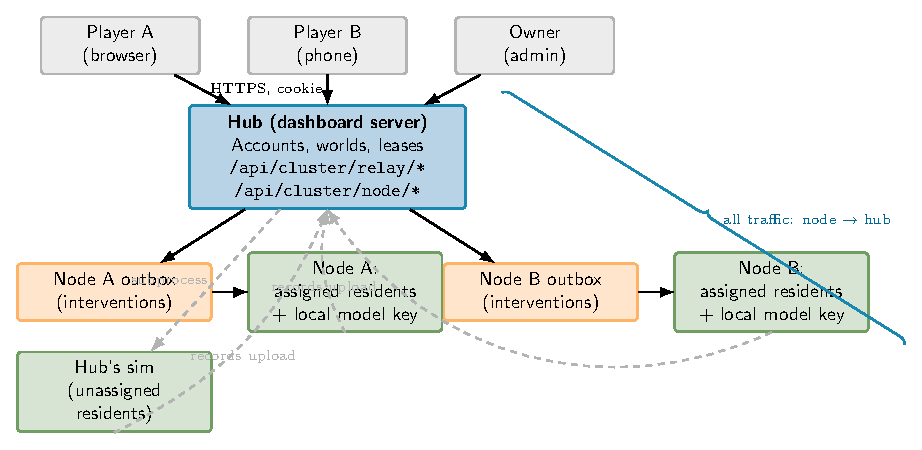
\includegraphics[width=\linewidth]{hub_node.pdf}
  \caption{Distributed playable topology.  The hub is the dashboard server;
  it owns accounts, the world metadata, the per-node outbox, the per-world
  relay, and the per-tenant Recorder merge.  Each node runs the simulation
  for its assigned residents, polls interventions, and uploads Recorder
  rows.  All cross-machine traffic is node-to-hub; the hub never opens
  inbound ports to a node.}
  \label{fig:hub-node}
\end{figure}

\subsection{Topology and threat model}

The topology is asymmetric on purpose: all traffic is node $\to$ hub.
Nodes can sit behind NAT, behind phone hotspots, or in a firewall; they
need only an outbound HTTPS connection to the hub.  This is a deliberate
trade-off: the protocol does not need a clock-synchronization primitive
because the hub does not advance simulation time.  Each node runs the
simulation locally; the hub merges per-node Recorder rows and routes
interventions.  No transactional consistency is offered; the protocol
is best-effort and tolerates brief disconnection.

The hub is the dashboard server; this means one port, one reverse proxy,
one TLS certificate for a public deployment.  The v1 standalone relay
(\texttt{distributed\_comm\_server}) is retained for OpenClaw-style
deployments, but in v2 it is no longer required: the dashboard server
embeds the relay as an in-process \texttt{DistributedRelayBackend}, one
per world.  The hub itself is also a node, identified as
\texttt{node\_id = hub}; it runs the simulation for residents that have
not been assigned to any external node, so that the world has at least
one heartbeat even when every external node is offline.

\subsection{Node lifecycle}

A node is added by the world's owner through the dashboard.  The owner
fills in a name (e.g., ``Lab 302 seat 7'') and a list of residents that
the node should run (either a list of ids or ``rebalance N'').  The hub
issues a one-time token of the form
$\texttt{world\_id}.\texttt{node\_id}.\texttt{secret}$, shows it once,
and stores the SHA-256 of the secret.  The secret is therefore a bearer
token; its revocation is immediate, and a revoked node receives a 401 on
its next heartbeat and stops the simulation.

The node process is a single Python command:

\begin{verbatim}
  python -m gaworld.cluster join <hub-url> --token <token>
\end{verbatim}

The node begins by sending a heartbeat.  The hub responds with
``world is running; new run id is \texttt{R}; please download the
world bundle''.  The node downloads a zip containing the world's
configuration, the seed \texttt{agents.csv} and \texttt{profiles.md},
and the city bundle.  It then launches the simulation subprocess with
\texttt{GAWORLD\_CONFIG\_OVERRIDES} carrying the world's configuration,
the per-node paths, the assigned residents, and the relay's URL and
token.  The simulation code does not change between local and remote
modes; only the override environment differs.

While the simulation runs, the node polls interventions every second,
enqueues them locally through the standard \texttt{kernel/remote}
interface, and the simulation drains the queue at the next tick as in v1.
The node also reads the per-table \texttt{records/*.jsonl} files every
second and uploads new rows to the hub, which appends them to the
world's merged Recorder with a \texttt{\_node} tag on each row.  When
the hub says ``stop'', the node terminates the subprocess; when the
subprocess exits on its own, the node reports that status in the next
heartbeat.  When the network is offline, the node keeps running and
back-fills records when the connection returns; when the simulation's
tick-sync timeout expires, the node advances without waiting.

\subsection{Player action routing}

A player intervention (\texttt{player\_claim}, \texttt{player\_act},
\texttt{player\_say}, or \texttt{player\_release}) is received by the
hub through the dashboard's \texttt{play} API.  The hub resolves the
intervention's target resident and routes it:

\begin{itemize}[leftmargin=*]
  \item If the resident is on the hub, the intervention is appended to
  the hub's local queue (as in v1).
  \item If the resident is on a remote node, the intervention is
  appended to that node's outbox; the next time the node polls
  (\textless 1 s in the v2 implementation), the intervention enters its
  local queue and is consumed at the next tick.
  \item For \texttt{player\_say}, the speaker and the listener may be on
  different nodes.  The speaker's node records ``you said X to Y'' as
  a local action; the listener's node receives a \texttt{player\_hear}
  intervention that adds ``Y said: X'' to the listener's next
  perception.
\end{itemize}

Player leases remain on the hub (\texttt{play\_api.\_CLAIMS}).  A
node's simulation does not need to know that the player exists; the
lease is the hub's bookkeeping, refreshed every 30 s.  If a node
disconnects, the lease remains valid on the hub and the player can
continue to be served; when the node reconnects, it re-registers any
active claims so the simulation can keep them consistent.

\subsection{Clock synchronization}

The hub and each node maintain a \emph{logical} clock that is updated
whenever a Recorder row arrives.  The simulation is allowed to advance
its own clock without coordination, so the protocol is not a
conservative-synchronization protocol: it tolerates drift.  Each node
periodically reports its clock to the hub, and the hub publishes a
\emph{median} clock that downstream code can use to align downstream
consumers (the visualizer, the Auditor UI, the intervention display).
The current implementation does not implement rollback or
deterministic-replay, and the protocol does not promise a
tighter-than-seconds clock alignment.  This is the trade-off that
makes the system operable behind NATs and is the reason the protocol
is best-effort.

\subsection{Security and access control}

Node tokens grant access to the per-world \texttt{/api/cluster/node/*}
and \texttt{/api/cluster/relay/*} endpoints; they do not grant access
to the dashboard, the account store, or to any other world.  Bearer
authentication is required for every request; the node id is bound to
the secret, and the secret is checked against a SHA-256 hash.  The hub
emits a structured audit row on every node request, including
``heartbeat'', ``bundle-download'', ``intervention-poll'',
``records-upload'', ``sync'', and ``denied''.  A revoked node receives
401 on its next request and stops the simulation.  When a node's
\texttt{node\_id} is reused after a restart, the new secret replaces
the old hash; the old secret is invalidated atomically.

\subsection{Deployment profiles}

A v2 deployment can be configured in three profiles:

\begin{itemize}[leftmargin=*]
  \item \textbf{Single tenant, single process} (v1-equivalent): accounts
  are off, the relay is in-process, and the only node is the hub.  This
  is the default for local research and for the bundled benchmarks.
  \item \textbf{Multi-tenant, single process}: accounts are on, the
  relay is in-process, and the only node is the hub.  This is the
  default for a classroom or workshop.
  \item \textbf{Multi-tenant, multi-node}: accounts are on, the relay
  is in-process, and one or more external nodes are connected.  This
  is the default for cross-machine deployments (a school lab, a
  cross-campus collaboration, a multi-region test).
\end{itemize}

The same code path runs in all three profiles; the differences are
configuration, not code.  A multi-node deployment does not promise
horizontal scalability, throughput improvement, or fault tolerance; it
promises the ability to assign residents to machines that have their
own model keys, and the ability to keep a world alive when one node
disconnects.

\section{Research and Counterfactual Workflow}
\label{sec:research-workflow}

GAWorld v2 treats an experiment as a configured execution that produces an
inspectable artifact tree, with each numeric result bound to a hash and an
evidence class.  The platform now exposes four research surfaces on top of
the underlying simulation: a matched-event workflow inherited from v1; a
parallel-worlds counterfactual engine; a Research Workbench that compiles a
paper or a research idea into a pre-registered protocol; and a
policy-simulation-and-optimization loop.  Each surface produces its own
artifact set and binds every result to the producing code path.  This
section describes the four surfaces; the Agent Playground and Arena are
covered separately in \cref{sec:playground-arena}.

\begin{figure}[t]
  \centering
  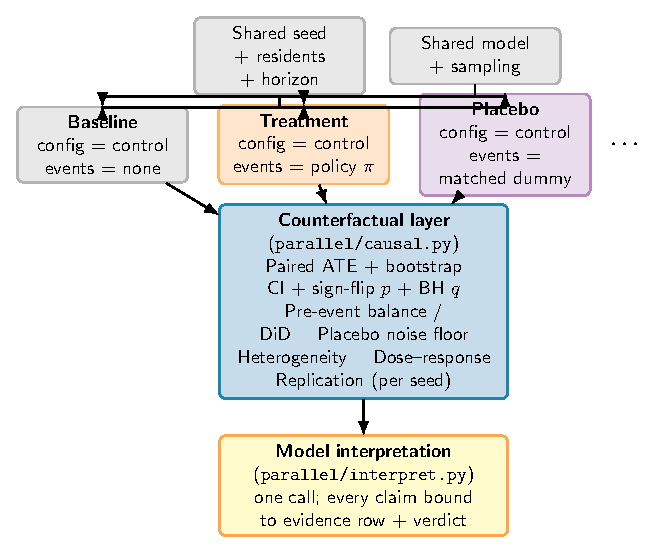
\includegraphics[width=\linewidth]{parallel_worlds.pdf}
  \caption{Parallel-worlds engine.  Up to eight matched worlds share the
  same seed, the same resident sample, and the same model.  Each world
  receives a per-world \texttt{config} patch and a per-world event list;
  the counterfactual layer then computes paired ATE, sign-flip $p$,
  pre-event balance, placebo noise floor, heterogeneity, dose--response,
  and replication.  An optional one-call model interpretation binds
  every claim to a specific evidence row.}
  \label{fig:parallel-worlds}
\end{figure}

\begin{figure}[t]
  \centering
  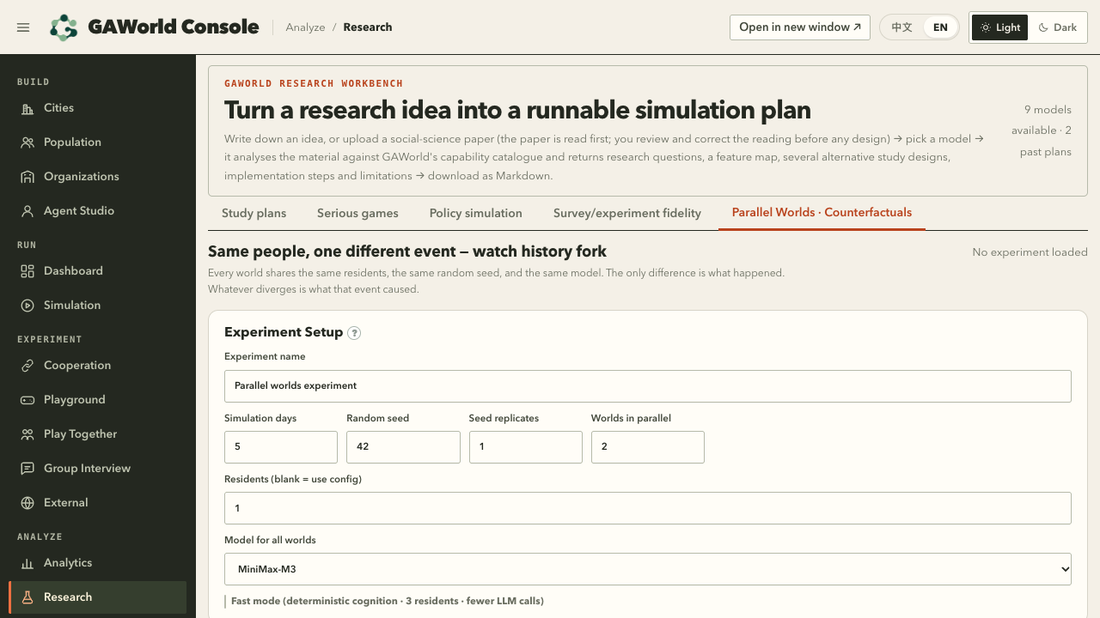
\includegraphics[width=\linewidth]{en_04_parallel.png}
  \caption{The Parallel Worlds tab.  A researcher fills in the experiment
  name, the simulation days, the random seed, the number of seed
  replicates (for the per-seed ATE and meta-analytic mean), the number of
  worlds to run in parallel (up to eight), the resident subset, and the
  model.  The \emph{Fast mode} toggle switches the engine to deterministic
  cognition with a smaller resident set so that the workflow can be
  rehearsed cheaply before a real run.}
  \label{fig:parallel-tab}
\end{figure}

\begin{figure}[t]
  \centering
  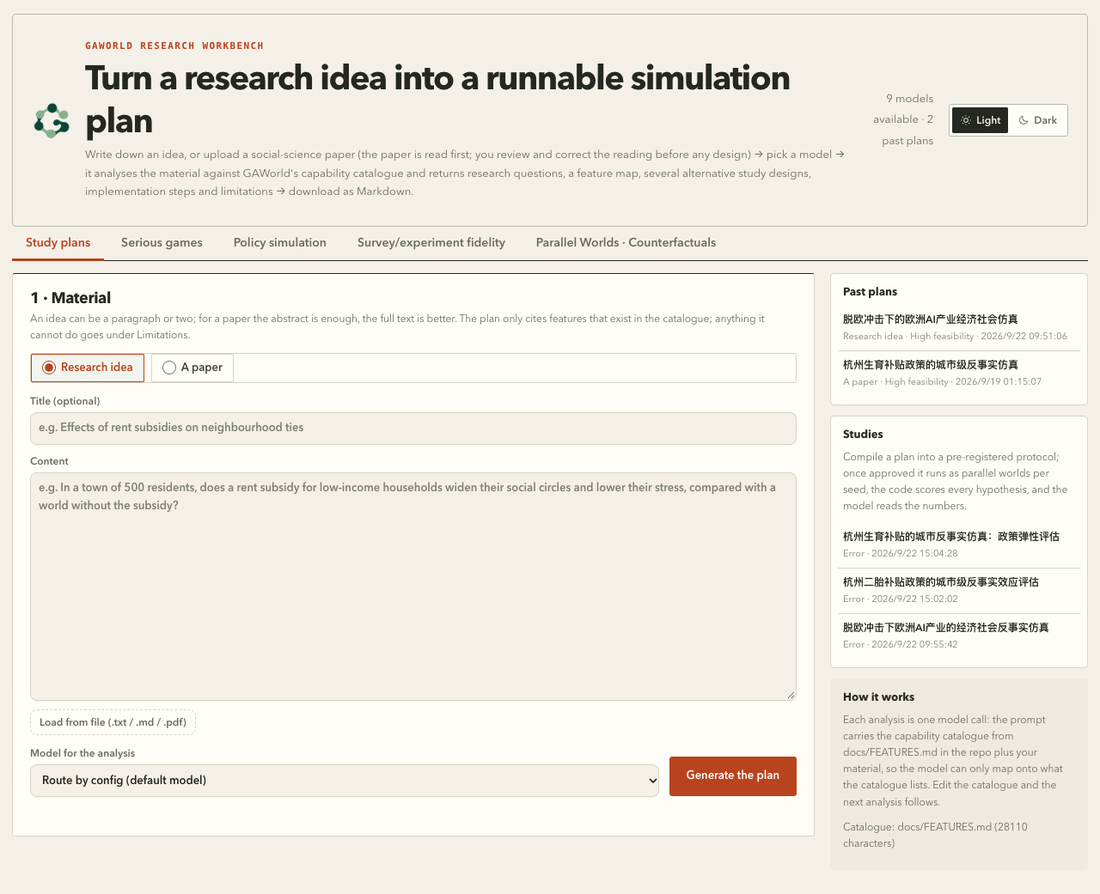
\includegraphics[width=\linewidth]{en_03_research.png}
  \caption{The Research Workbench.  A researcher pastes a research idea
  or uploads a paper, picks a model, and the system returns a plan: a
  theory, a methods paragraph, key variables, hypotheses, a feature map
  to the GAWorld surface, two or three experimental designs, and a list
  of limits.  The plan is editable; the model cannot write to a feature
  that is not in \texttt{FEATURES.md}, and the protocol compiler cannot
  use a metric that is not in the \emph{measurable catalog}.  The
  \emph{Study plans}, \emph{Serious games}, \emph{Policy simulation},
  \emph{Survey / experiment fidelity}, and \emph{Parallel Worlds
  Counterfactuals} tabs reuse the same pane to compile plans, run
  serious-game sessions, and run paper-fidelity studies.}
  \label{fig:research-workbench}
\end{figure}

\begin{figure}[t]
  \centering
  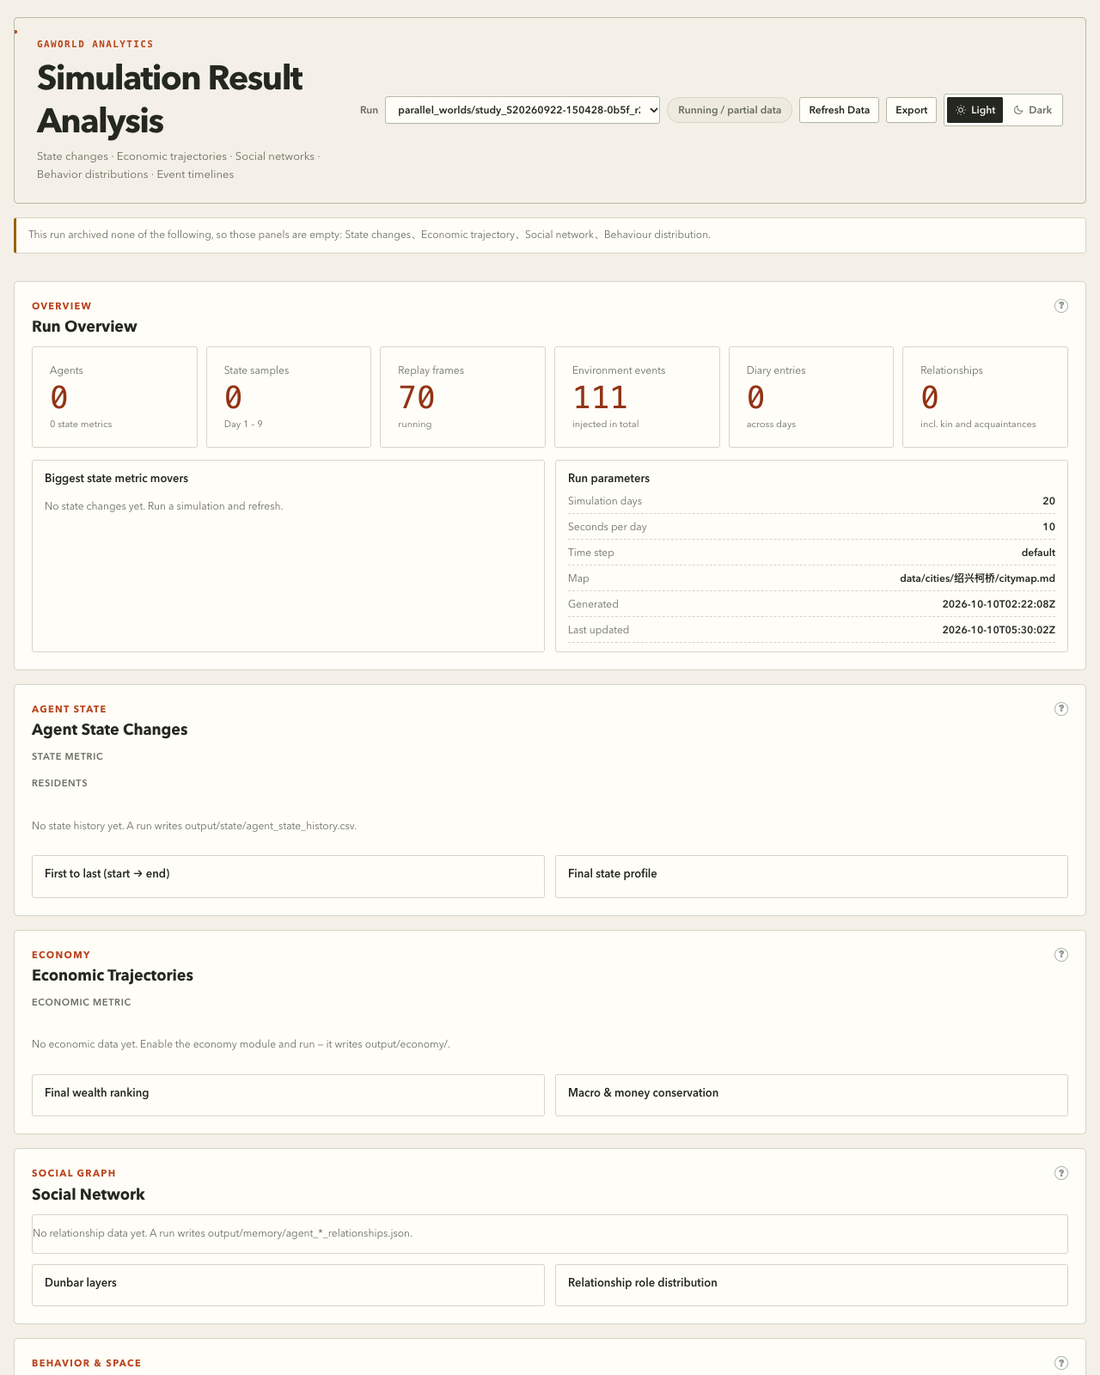
\includegraphics[width=\linewidth]{en_09_analytics.png}
  \caption{The Analytics pane.  After a run, the analytics pane exposes
  per-run counts (agents, state samples, replay frames, environment
  events, diary entries, relationships), a per-day event timeline broken
  down by source (\emph{social / natural / economic / political /
  life\_event / technology}), an event-type distribution, and an
  impact-tag distribution.  When a run is incomplete or a metric is
  missing, the pane displays \emph{No data yet} in the corresponding
  block rather than fabricating a value, in line with the evidence-class
  policy.}
  \label{fig:analytics}
\end{figure}

\subsection{Matched event and baseline runs}

For intervention studies, the \texttt{compare-event} command constructs two
scenario directories under a timestamped comparison root.  The
\texttt{without\_event} arm inherits the configured policy-event list, whereas
the \texttt{with\_event} arm appends a named event at an explicit simulation
day and clock time.  Both arms receive the same requested agent subset,
simulation horizon, random seed, and---when supplied---LLM provider override.
Before execution, each arm is reset within its own isolated memory, log,
vector-database, state, network, environment, intervention, and visualization
directories.  The two runs are then launched concurrently.  This organization
reduces accidental cross-arm state leakage and makes missing or failed arms
visible through separate reset and run logs.

After both subprocesses finish, the comparison routine reads each arm's
\texttt{state/agent\_state\_history.csv}.  For every available metric, it
computes the across-agent final snapshot, the mean over recorded observations,
and event-minus-baseline differences.  Machine-readable results are stored in
\texttt{comparison\_metrics.csv}; \texttt{comparison\_summary.md} provides a
human-readable view.  The separate \texttt{run\_meta.json} records choices
such as seed, horizon, provider, world identifier, node identifier, and
whether the lower-fidelity fast mode was requested.  v2 adds a
\texttt{warnings.json} that records any plugin or stage that failed to load
and the active plugin list; this makes the artifact self-describing about
which mechanisms were actually present.

\subsection{Parallel worlds and counterfactual inference}

The parallel-worlds engine generalizes the matched-event workflow.  An
\emph{experiment specification} describes up to eight worlds, a shared seed,
a per-world \texttt{config} patch, a per-world event list, and (optionally) a
set of replication seeds.  The engine runs the worlds sequentially under a
shared \texttt{GAWORLD\_CONFIG\_OVERRIDES} skeleton; the seed and the patch
together determine the per-world trajectory.  Per-arm completion status is
recorded in \texttt{worlds/<id>/run\_meta.json} and the per-arm artifact
trees are kept separate so that one arm's failure cannot contaminate another.

After all arms complete, the inference layer (\texttt{parallel/causal.py})
computes a deterministic counterfactual summary from the recorded state
trajectories.  No model call is made during inference.  The summary
includes:

\begin{itemize}[leftmargin=*]
  \item \textbf{Paired per-resident ATE} with a bootstrap confidence interval
  and a sign-flip $p$-value, for every metric that both arms recorded;
  \item \textbf{Pre-event balance} and a difference-in-differences estimator
  that uses the matched pre-event window as a baseline;
  \item \textbf{Placebo noise floor}: a separate placebo comparison that
  shows how large a difference arises from no intervention at all, with the
  same seed;
  \item \textbf{Onset order} and \textbf{heterogeneity}: the step at which
  the two trajectories first diverge and the per-resident effect size
  distribution;
  \item \textbf{Dose--response} for design points that vary an intervention
  parameter across worlds;
  \item \textbf{Replication} across seeds, with a per-seed ATE and a
  meta-analytic mean; and
  \item \textbf{Multiple-testing correction} with Benjamini--Hochberg
  $q$-values.
\end{itemize}

A study verdict is a function of the deterministic summary: a hypothesis is
\emph{supported} if its signed effect has $q<0.05$ and the replication mean
agrees in sign; \emph{reversed} if the sign agrees but the effect is
negligible; \emph{undetermined} if the replication is mixed; and
\emph{unmeasured} if the producing metric is missing in either arm.
The verdict gate is part of the same code path that the v1 GAWorld-Bench
used, so the meaning of a verdict is consistent across the two surfaces.

An optional one-call model interpretation (\texttt{parallel/interpret.py})
follows the inference.  The model sees the inference summary and the
per-comparison verdict and produces a brief narrative; every claim in the
narrative is bound to a specific evidence row and a verdict, and the
interpretation is cached per comparison so that reruns are deterministic
modulo provider noise.  v2 does not allow the model to overturn a
deterministic verdict: the verdict is the verdict.

\subsection{Research Workbench: from a paper or idea to a protocol}

The Research Workbench \citep{gaworldbench} divides a study into a planning
phase (output: a plan document) and an execution phase (output: a verdict
and a report).  The planning phase is a \emph{plan generator} that takes
either a research idea in free text or a paper (URL or PDF) and emits a
\emph{plan} with a theory, a methods paragraph, key variables, hypotheses,
a feature map to the GAWorld surface, two or three experimental designs,
an implementation outline, a credibility plan, and a list of limits.  The
plan is editable; the model cannot write to a feature that is not in
\texttt{FEATURES.md}, and the protocol compiler cannot use a metric that
is not in the \emph{measurable catalog}.

The execution phase is a \emph{protocol compiler} that takes the chosen
design and produces a \emph{pre-registered protocol}: a list of
conditions, a list of outcomes with pre-specified effect directions and
minimum effect sizes, a list of pre-registered exclusion rules, and a
list of confidence-thresholds.  A pre-execution check
(\texttt{research/evaluate.py}) verifies the protocol against the
measurable catalog and refuses to start a study that fails the check.
After the study runs, the deterministic verdicts are compared with the
pre-registered expectations; an \emph{unexpected} verdict is reported as
such and is not rewritten to look like the prediction.  The final
report contains the pre-registered protocol first, then the results,
then the interpretation, in that order.  This pattern follows the
spirit of the recent pre-registration literature in computational
social science and is intended to discourage post-hoc rewriting.

\subsection{Policy simulation and optimization}

The policy-simulation loop \citep{gaworldpolicy} takes a description of a
policy (and, optionally, a candidate version) and a fixed-scale sample of
residents, and produces a JSON reaction per resident.  The deterministic
scoring aggregator converts the residents' JSON into a composite score.
v2 then optionally calls a model with the score and the policy to propose
modifications; the modified policy is re-simulated on the same resident
sample, and the policy with the highest composite score is the
recommendation.  This is an \emph{optimization} in the sense that the loop
produces a candidate that scored higher than the original on the
deterministic composite; it is not a guarantee that the higher score
reflects a better real-world policy.  The loop is bounded by a maximum
number of iterations and by a hard cap on the number of LLM calls; the
artifact records both budgets and the policies it produced.

\subsection{Serious games and workshop studies}

The \emph{serious-game} module \citep{gaworldseriousgame} is a turn-based
role-play surface in which two or more roles are seated by a resident
agent or a human through a seat link.  Each round, the seated participants
respond simultaneously; a facilitator call resolves the round; a debrief
scores each role on a fixed rubric.  Designs and sessions are stored under
\texttt{output/research/serious\_games/} and re-loadable for inspection.
The serious-game surface is intended for participatory studies in which
the researcher wants to see how a human participant negotiates with
simulated residents under a fixed scenario; it is not a high-throughput
evaluation surface and is not used for benchmark scoring.

\subsection{Group interviews and persona distillation}

A \emph{group interview} is a one-shot elicitation across a roster of
residents, run as a child process per city and aggregated in the dashboard
\citep{gaworldinterview}.  Each resident answers a fixed set of questions
and the result is written to \texttt{output/interviews/<session\_id>/}
together with the resident's response, the producing code path, and the
model and seed that produced the answer.  A \emph{persona distillation}
takes a name or a URL and produces a sourced portrait (identity, state,
Big-Five, mental models, expression DNA, limits) that can be deployed as a
resident; the portrait and the producing research notes are stored under
\texttt{output/personas/<slug>/} and only \emph{deploy} writes the seed CSV
\citep{gaworldpersona}.  The deploy step is a separate, reviewed action
that the system refuses to perform automatically, so that an unverified
portrait cannot enter a population.

\subsection{What the workflow identifies}

The four surfaces above are useful scaffolds for counterfactual
experiments, but the recorded differences are still single contrasts
produced by an LLM-mediated dynamical system.  A common seed does not
guarantee common latent randomness after prompts diverge, and a policy
description does not guarantee that an economic or mobility mechanism
changed.  Before interpreting a difference, a researcher should verify
the intervention's path from event to structural state, replicate both
arms over seeds, pre-register target metrics, and include placebo events
or negative-control outcomes \citep{lipsitch2010negative}.  External
policy conclusions additionally require a defensible mapping to the
population and institutions of interest.  GAWorld v2 currently supports
constructing and auditing such a study, not replacing it.  The
deterministic verdict gate and the per-arm completion audit make a
defensible study easier to perform than the v1 system made it, but they
do not make a non-defensible study a defensible one.

\section{Agent Playground and Arena}
\label{sec:playground-arena}

Beyond the research surfaces, v2 ships two evaluation surfaces that probe
residents on a smaller scale.  The Agent Playground is a library of
fourteen game-based probes; the Agent Arena is a benchmark harness.  Both
surfaces are \emph{in-memory} by default, write only their configured
archives, and never modify a city bundle.  They are designed to make a
small group of residents answer a structured question in a way that can be
inspected, replayed, and scored under deterministic rules.

\begin{figure}[t]
  \centering
  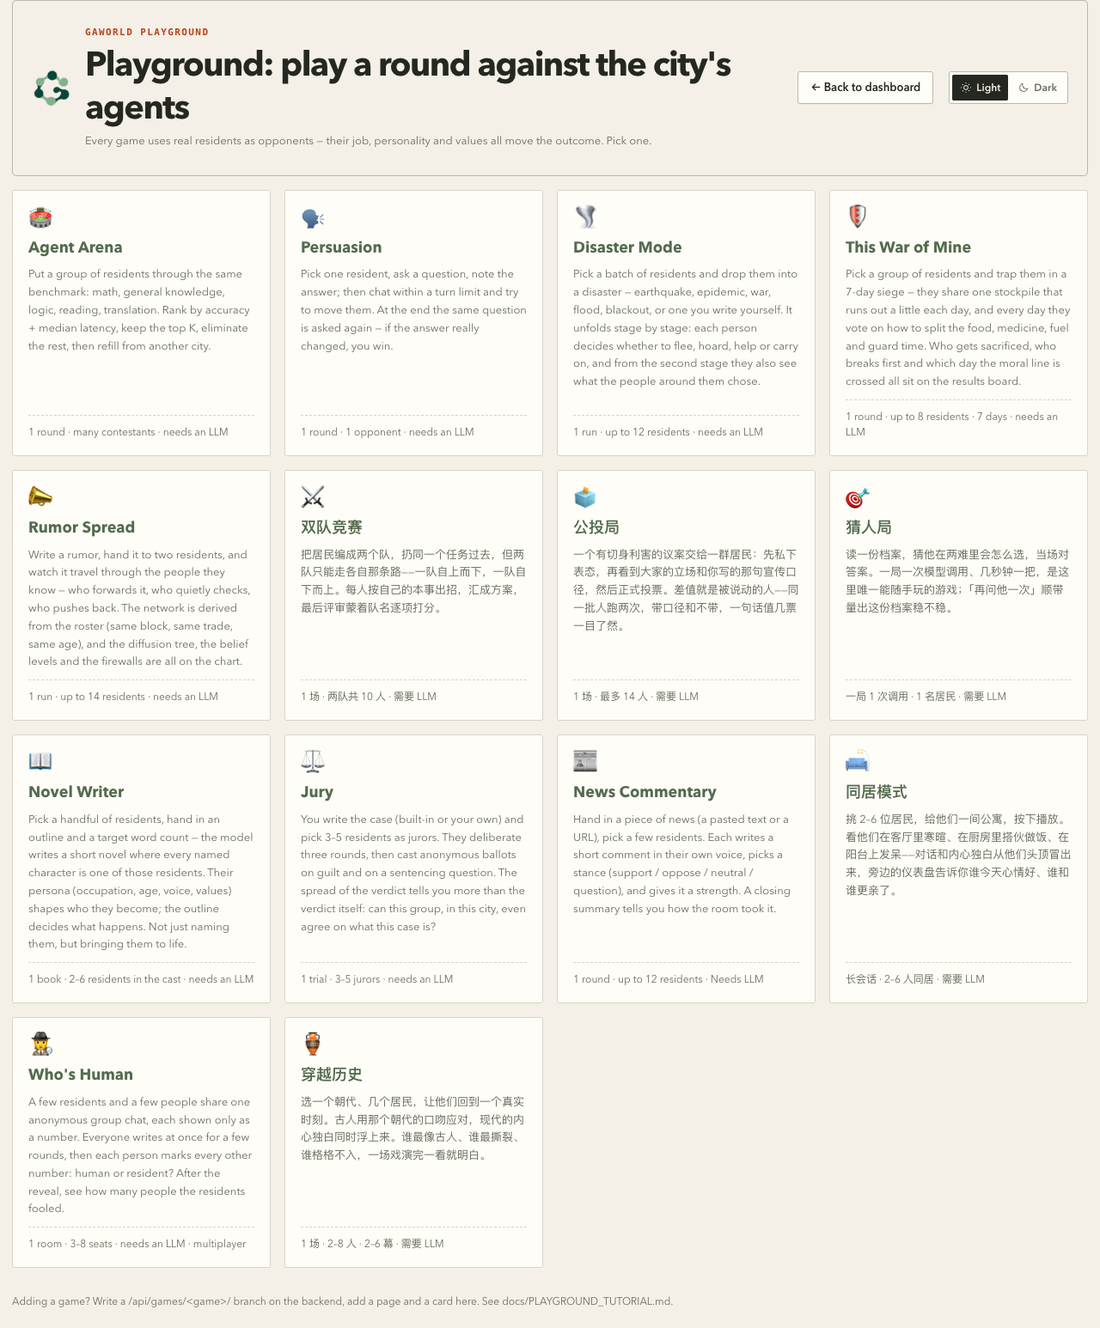
\includegraphics[width=\linewidth]{en_05_games.png}
  \caption{The Agent Playground.  Each card is a game-based probe; the
  fourteen cards in the v2 set cover the four families
  (one-on-one, one-group-one-event, mission / creative, and
  long-form / human-in-the-loop).  Every card is a deterministic
  harness over a real resident's response; per-game archives are
  written to \texttt{output/games/<game>/} on completion and feed
  the Track B scorecard.}
  \label{fig:playground}
\end{figure}

\begin{figure}[t]
  \centering
  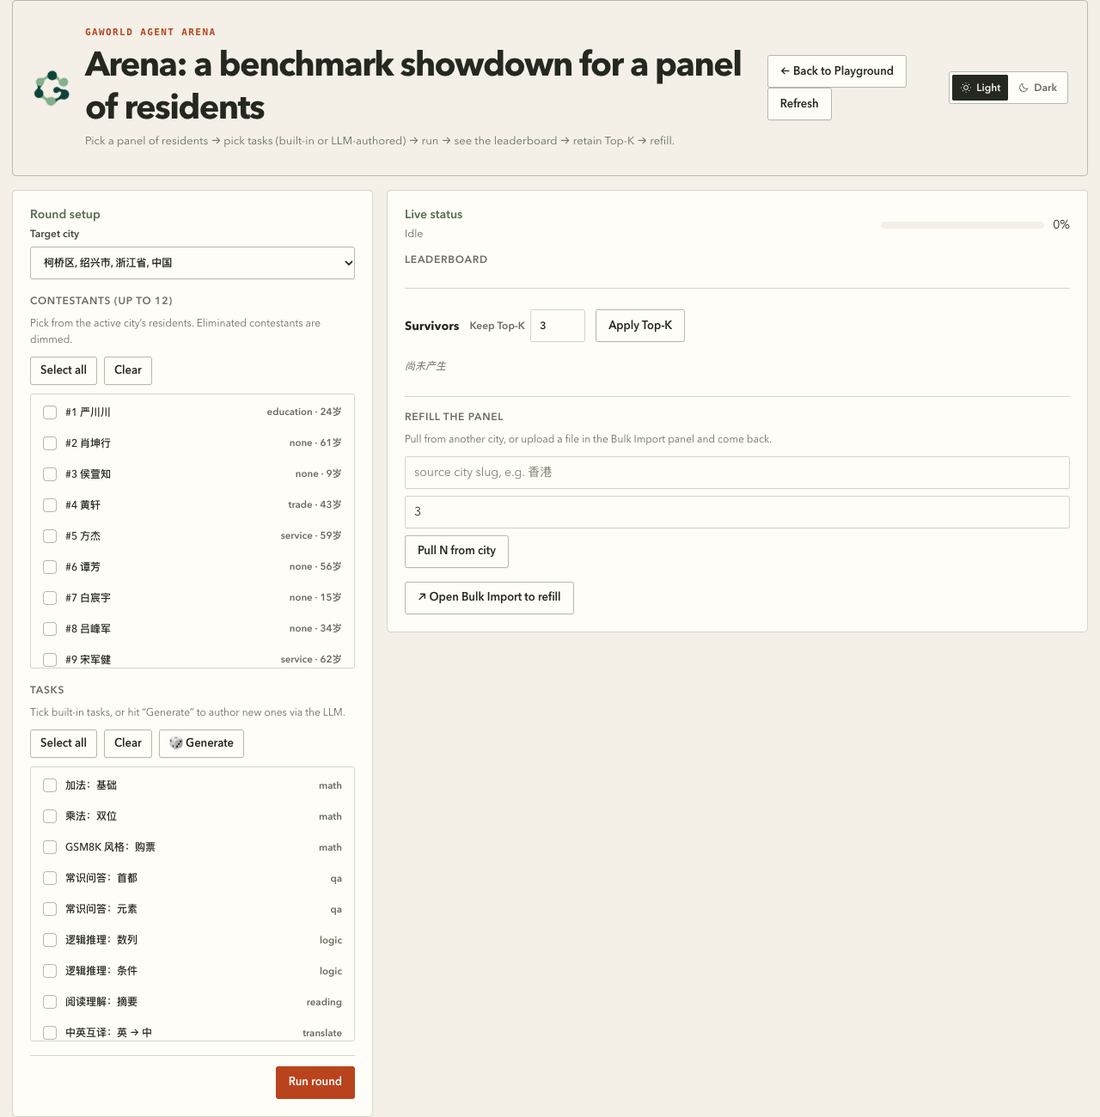
\includegraphics[width=\linewidth]{en_06_arena.png}
  \caption{The Agent Arena.  A researcher picks a target city, a panel
  of up to twelve residents, and a question set (a built-in bank of
  ten questions or an LLM-generated set).  After the round, the
  leaderboard ranks the residents by correctness and median latency.
  A \emph{Keep Top-K} policy retires the bottom of the panel; the
  \emph{Refill the panel} controls pull new residents from another
  city or from a bulk-import file.}
  \label{fig:arena}
\end{figure}

\subsection{The fourteen game families}

The Agent Playground \citep{gaworldplayground} covers four broad families,
grouped by the kind of evidence the probe produces.  Each game has a
deterministic scoring rule that does not depend on a judge's LLM call,
and a \emph{judge} layer for the games whose scoring is genuinely
qualitative.  The four families are:

\begin{itemize}[leftmargin=*]
  \item \textbf{One-on-one}.  \emph{Persuasion}: a researcher asks a
  resident a question, has a brief conversation, and re-asks; the judge
  model compares the first and last answer to decide whether the resident
  changed their mind.  \emph{Read the room}: a resident is given a moral
  dilemma and asked to predict what another named resident would do; the
  scoring rule is exact match to the named resident's actual response.
  \emph{Jury}: three to five residents hold a three-round discussion, vote
  anonymously, and decide on a sentence; the verdict is the majority, not
  the judge model.
  \item \textbf{One group, one event}.  \emph{Disaster mode}: a group of
  residents passes through a disaster stage by stage; each resident
  produces a structured JSON (action, panic, help, quote); the histogram
  is deterministic.  \emph{Warzone}: when a warehouse runs low, residents
  propose and vote on a daily basis; mortality, the Gini coefficient, and
  the vote-disagreement rate are all deterministic.  \emph{Rumor spread}: a
  rumor is seeded, the model picks a verb (forward / verify / refute /
  ignore), the graph picks a recipient, and the run produces a propagation
  tree.  \emph{Referendum}: a self-interested bill is voted on privately
  and then publicly; an optional propaganda paragraph can be inserted; the
  shift in public opinion is reported.  \emph{News commentary}: a news
  item is shown to one to twelve residents who each produce a single
  comment with a stance and an intensity.
  \item \textbf{Mission / creative}.  \emph{Team duel}: two teams work on
  the same task from opposing angles; reviewers blinded to team name score
  on dimensions.  \emph{Novel writer}: two to six residents become
  protagonists of a single novel with an outline.
  \item \textbf{Long-form / human-in-the-loop}.  \emph{Roommate mode}:
  two to six residents share a virtual apartment; the front-end polls
  the simulation each tick.  \emph{Who's human}: residents and a real
  human sit in an anonymous group chat; the human enters through a seat
  link.  \emph{Timeslip}: two to eight residents are dropped into a real
  dynasty's decisive moment; each round produces an era-styled line and a
  modern inner monologue; a three-axis rubric (era fit, stability, inner
  conflict) is deterministic.
\end{itemize}

This is a heterogeneous set.  Some games are deterministic given the
residents' responses (\emph{warzone}, \emph{rumor}, \emph{referendum},
\emph{disaster mode} for its histogram), some depend on a judge LLM
(\emph{persuasion}, \emph{team duel}, \emph{novel writer}), and some are
genuinely participatory (\emph{who's human}, \emph{roommate mode}).  The
common interface is a fixed rule for routing, scheduling, and archiving;
the scoring rules differ and are documented per game.

\subsection{Archives and the Track B scorecard}

A subset of games (\emph{rumor spread}, \emph{referendum},
\emph{disaster mode}) writes an archive to
\texttt{output/games/<game>/<timestamp>-<job\_id>.json} on completion.
The archive contains the per-resident response, the round-by-round state
(if any), the deterministic scoring result, the model that produced each
response, and the user that initiated the run (in a multi-tenant
deployment).  These archives are the data source for the
\emph{GAWorld-Bench Track B} scorecard, which checks three pre-registered
laws (``referendum conformity'', ``disaster solidarity > panic'', ``rumor
decline after refutation, but not to zero'').  Each law is tested with at
least five runs; if fewer than five usable runs are available, the law
is reported as \emph{withheld} and not as \emph{supported} or
\emph{reversed}.  Track B is therefore a structured way to combine
across-game evidence under a pre-registered rubric, distinct from Track A
which is a software-path diagnostic.

\subsection{Agent Arena}

The Agent Arena is a benchmark harness for a fixed set of residents
\citep{gaworldarena}.  The arena takes a target city, a set of residents
(up to twelve), and a question set.  A question set is either a built-in
bank of ten questions covering math, QA, logic, reading, and translation,
or an LLM-generated question set of arbitrary size, difficulty, and
category.  Each resident answers each question; the score is correctness
and median latency.  A researcher can apply a Top-$K$ retention policy
and the residents outside the top $K$ are marked as \emph{retired}; the
researcher can also pull new residents from another city or from a
batch-import file to replace the retired residents.

The arena is \emph{not} a population benchmark.  It does not produce a
statement about the model's overall ability, only about a small set of
named residents under a specific question bank.  This restriction is
deliberate: residents in GAWorld are not interchangeable with each other,
and a benchmark that mixed their identities would not produce
interpretable evidence.  The arena's archive is per-resident and
per-question, and it is the researcher's responsibility to compare
results across cities or across model configurations in a defensible way.

\subsection{State and ownership}

A game session is held in memory; the dashboard exposes a ``recent
sessions'' panel that displays the last twenty sessions.  The
\texttt{JobStore} for game sessions is per-game, in-memory, and is
discarded when the dashboard restarts.  Archives, by contrast, are
persisted to \texttt{output/games/<game>/} and survive restarts.  In a
multi-tenant deployment, every archive is stamped with the world
identifier and the user that initiated the run.  Game state is not part
of the city bundle and is never written to it; the only side effect on
the bundle is the existence of an agent (and that effect comes from the
underlying city, not from the game).

\subsection{What the games evaluate}

The Agent Playground is a probe layer, not a population benchmark.  Its
value is in producing per-game archives that can be inspected and
compared across runs, and in providing a small set of pre-registered
laws that the Track B scorecard tests.  The games do not establish that
the residents are realistic, that the underlying model is a good
representative of a population, or that the scoring rules are calibrated
against human behavior.  A finding in Track B is therefore a hypothesis
about how the residents behave under a structured scenario, not a
generalization to a real population.  This is the same validation
posture as the v1 system paper's Track A: the harness is a software
artifact, the evidence it produces is a per-game archive, and the
verdict is a deterministic function of the archive.

\section{Existing Capability Cases}
\label{sec:capability-cases}

This section audits what the archived v2 outputs demonstrate about
GAWorld as a research instrument.  It does not treat an available file as
a successful scientific evaluation.  We use the v2 evidence classes:
\textsf{REAL} for a usable GAWorld run artifact; \textsf{DIAGNOSTIC} for
a re-analysis of a \textsf{REAL} artifact; \textsf{SYNTHETIC} for a
fixture produced by \texttt{-{}-synthetic}; \textsf{INCOMPLETE} for a
missing, interrupted, or insufficient output; \textsf{DESIGNED} for a
protocol that exists without usable outcome evidence; and \textsf{FIXTURE}
for synthetic data that tests analysis code.  These labels describe
evidence availability, not system performance.

\begin{figure}[t]
  \centering
  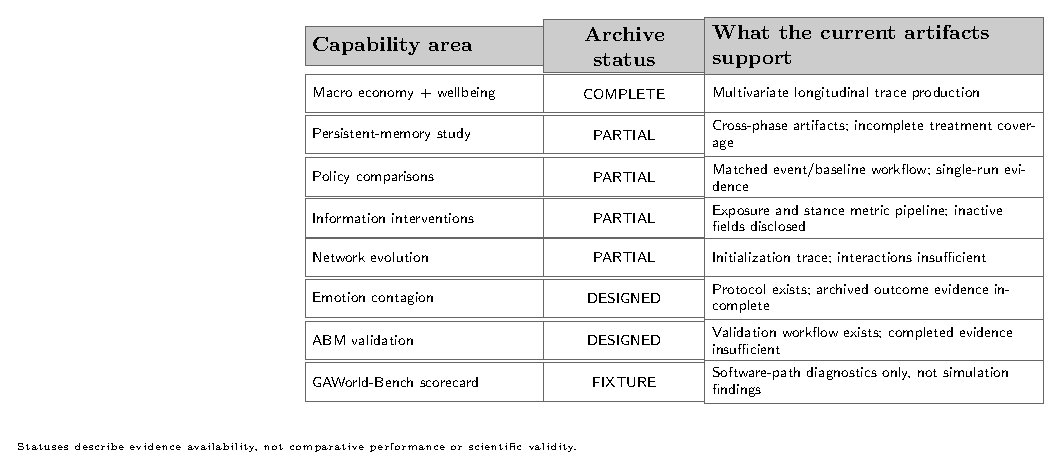
\includegraphics[width=\linewidth]{capability_matrix.pdf}
  \caption{Coverage of the audited v2 result archive.  The matrix
  distinguishes inspectable capability evidence from incomplete
  evaluations and diagnostic fixtures; it is not a leaderboard or a
  validation score.}
  \label{fig:capability-matrix}
\end{figure}

\begin{table}[t]
\centering
\small
\caption{Status of all experiment families represented in the v2
artifact ledger.  Counts and horizons describe the archived files, not a
common evaluation protocol.}
\label{tab:archive-status}
\begin{tabular}{@{}p{0.22\linewidth}p{0.16\linewidth}p{0.22\linewidth}p{0.32\linewidth}@{}}
\toprule
Area & Status & Archived scope & Permitted use \\
\midrule
Macro economy and wellbeing & \textsf{REAL} & $n=5$ agents, one seed, three-day configuration; 116 recorded steps per agent & Multivariate state-trace production, not an economic or psychological finding \\
Persistent memory & \textsf{INCOMPLETE} & $n=1$ agent; four planned 14-day arms; only one completed both seven-day phases & Persistence and cross-phase artifact inspection, not a treatment comparison \\
Policy comparisons (v1 archive) & \textsf{REAL} & Four single archived event--baseline pairs; Day-3 events; no seed replications & Pairing, isolation, and metric extraction, not policy effects \\
Information intervention & \textsf{INCOMPLETE} & Three arms, $n=5$ each; unequal horizons of one or two days & Information-metric schema and missing/inactive-field audit \\
Polarization & \textsf{INCOMPLETE} & Two arms with 109 versus 85 records & Availability of a comparison artifact; unequal records preclude an effect claim \\
Network evolution & \textsf{INCOMPLETE} & $n=5$, 14-day report; zero recorded interactions on every day & Initialization and failure visibility, not emergent-network evidence \\
Emotion contagion & \textsf{INCOMPLETE} & Four intended arms; all four report a missing state-history file & Protocol coverage only; no outcome result \\
ABM validation & \textsf{INCOMPLETE} & Validation workflow is present; completed empirical evidence is insufficient & Evaluation design only, not an empirical validation result \\
GAWorld-Bench Track A & \textsf{FIXTURE} & Built-in synthetic scorecard & Parser and scoring-path diagnostics only \\
GAWorld-Bench Track B (rumor / referendum / disaster) & \textsf{REAL}, \textsf{INCOMPLETE} & A handful of per-game archives; not enough runs to test the three pre-registered laws & Probe library, not population evidence \\
Parallel-worlds sweeps & \textsf{DIAGNOSTIC} & Cached per-arm artifact trees from a recent transport-restriction sweep & Counterfactual-inference code paths; not policy evidence \\
Multi-tenant isolation & \textsf{REAL} & Two-world deployment with a single dashboard, two world roots, two Recorder streams & Isolation mechanics, not scale claim \\
Distributed playable city & \textsf{REAL} & Two-node + hub deployment with one world, residents split between hub and node, player interventions routed across nodes & Hub-node protocol mechanics, not throughput claim \\
Persona distillation & \textsf{REAL} & One distilled portrait, one deployed resident & Distill-and-deploy workflow, not population claim \\
\bottomrule
\end{tabular}
\end{table}

\subsection{Case 1: Persistence is observable, but the memory contrast is not}

The memory-consistency archive is useful because it exposes a longitudinal
experimental shape that is often hidden in agent demonstrations.  One agent
(ID 34) was assigned to four intended treatments: intact memory, reset
between phases, selective summary deletion, and injected conflict.  Each
arm planned a seven-day acquisition phase followed by a seven-day
continuation phase.  The archive contains seven phase-1 diaries for every
arm, together with state and memory files.  It also records different
memory-file footprints, including episodic, growth, habit, and
relationship artifacts.  Thus a researcher can inspect what persisted, what
was deleted, and how a later elicited action was represented.

Only the intact-memory arm, however, contains all seven phase-2 diaries.
The reset, selective, and conflict arms each stop after phase 1, with the
archived report attributing the interruption to initialization after the
worker pool started.  The archive therefore demonstrates file-backed
persistence across two phases for one agent in one arm; it does not
compare the behavioral effect of memory retention, deletion, or conflict.
Qualitative labels such as a move from ``procrastinating'' to ``active''
are post-hoc codings of a few generated actions, not a validated
continuity measure.  In particular, differences in phase-1 final actions
cannot explain missing phase-2 outcomes.  This failure is scientifically
informative at the infrastructure level: treatment completeness must be
checked before interpreting a fluent diary as longitudinal evidence.

\subsection{Case 2: Policy artifacts exercise a counterfactual workflow}

The v1 policy archive contains four timestamped comparisons---traffic
restriction, housing subsidy, medical reimbursement, and job-training
subsidy.  Each stores an event arm beside a baseline arm and exports the
same metric columns, thereby exercising the isolation and reduction path
described in \cref{sec:research-workflow}.  All are single archived
comparisons, with events injected on simulation day 3 (09:00 for traffic
and 08:00 for the other three); there is no multi-seed sampling
distribution or uncertainty estimate.

The raw CSV files also show why mechanistic inspection must precede
substantive interpretation.  In every pair, the final values of
\texttt{cross\_viewpoint\_exposure}, \texttt{misinformation\_risk},
\texttt{stance\_score}, and \texttt{toxicity\_score} are zero in both
arms.  Some generic state variables differ: for example, the housing
comparison has a final event-minus-baseline \texttt{time\_pressure}
difference of $-0.0311$ and the traffic comparison a
\texttt{mobility\_intent} difference of $-0.0036$.  These numbers are
reported only to show that the reducer retains metric direction and
magnitude.  A single LLM-mediated trajectory cannot tell whether the
named policy caused the difference, whether the relevant structural
mechanism was connected, or whether the sign would persist under a new
seed.  The case supports a workflow claim---GAWorld can preserve paired
trees and compute declared contrasts---rather than a claim about
housing, health, training, or transport policy.

\subsection{Case 3: Information metrics make inactivity visible}

The misinformation artifact contains three five-agent arms.  The control
and treatment B each cover two simulated days, whereas treatment A covers
one.  Across every recorded day and arm, average misinformation risk is
$0.0$, and the reported peak and final risks are also $0.0$.  Mean
cross-viewpoint-exposure is $0.06656$ for control, $0.06707$ for
treatment A, and $0.06635$ for treatment B.  The unequal horizons rule
out a balanced comparison, and differences at the fourth decimal place
are descriptive properties of these files, not estimated intervention
effects.

That negative result is nevertheless a useful system diagnostic.  The
archive records treatment names, horizons, agent counts, daily risk
series, and an exposure aggregate together.  It does not prove that
misinformation propagated, that risk detection was sensitive, or that
the interventions changed exposure.  The separate polarization artifact
reinforces the boundary: its two arms contain 109 and 85 records,
respectively, and thus cannot be read as a balanced longitudinal
contrast without reconstructing the missingness.  v2's value here is
inspectability---inactive fields and unequal coverage remain visible
rather than being silently converted into a success score.

\subsection{Case 4: Economy--wellbeing traces provide dense state, not external validity}

The macro-economy archive is the most complete artifact for demonstrating
multivariate trace production.  Its hashed long-format CSV contains
11{,}600 rows for five agents, 116 unique recorded steps per agent, and
20 metrics per step ($5\times116\times20$).  The associated
configuration describes a three-day, seed-42 run.  Direct aggregation of
the CSV gives 580 values for each metric across agents and steps.  Mean
emotion, stress, and economic security are $0.4896$, $0.5490$, and
$0.6270$, respectively; their observed ranges are $[0.0233, 0.9310]$,
$[0.0907, 0.9898]$, and $[0.4455, 0.8298]$.

The raw row count matters because the accompanying narrative report
describes ``580 timesteps per agent.''  In the CSV, 580 is instead the
number of agent--step values for one metric ($5\times116$); each agent
has 116 distinct step identifiers.  We therefore use the CSV
cardinalities rather than the report's timestep wording.  This
discrepancy illustrates the role of an artifact ledger: even a plausible
derived report must be checked against its hashed source.

The trace can support new descriptive analyses without a new simulation.
For example, partitioning the 116 step identifiers into consecutive
ranges $0$--$38$, $39$--$76$, and $77$--$115$ yields emotion means of
$0.6365$, $0.5020$, and $0.3305$, while stress means are $0.4122$,
$0.5428$, and $0.6916$.  These bins are equal-index summaries, not
validated ``days,'' and the trajectories remain generated state
variables from one seed.  They show that GAWorld records joinable,
time-indexed state across agents and constructs; they do not show
human wellbeing dynamics, economic realism, or an effect of any
real-world shock.  v2's price-level multiplier is enabled in this
archive; the wage index is disabled, and the legend records that
omission.

\subsection{Case 5: Multi-tenant isolation mechanics}

A two-world deployment (one \emph{private}, one \emph{open}) was used to
audit the K6 migration.  The \emph{private} world is owned by
\texttt{alice} and is invisible to \texttt{bob}; the \emph{open} world
is owned by \texttt{alice} and lets \texttt{bob} join as a player.  Both
worlds run simultaneously; their \texttt{output/} trees are disjoint;
their Recorder streams carry distinct \texttt{\_node} tags when the hub
is also a node.  The artifact ledger shows that \texttt{alice}'s
mutation in the \emph{private} world did not affect \texttt{bob}'s
\emph{open} world and that \texttt{bob}'s player intervention in the
\emph{open} world was routed to the right node within the poll interval.
The audit does not establish a multi-tenant throughput claim: the
two-world deployment is a fixture for the isolation mechanics, and a
real classroom deployment is needed to exercise the FIFO queue, the
per-tenant quota, and the static-file guard.  The ledger records this
explicitly.

\subsection{Case 6: Distributed playable city mechanics}

A two-node + hub deployment was used to audit the K7 migration.  The
hub ran the dashboard, the account store, and the residents assigned
to it; one external node ran the remaining residents with the node's
own model key.  A player (\texttt{carol}) joined the \emph{open} world
through the browser, claimed a resident on the external node, and
performed three interventions over a 30-second window.  The artifact
ledger shows that each intervention was routed to the right node
within the poll interval, that the resident's next perception included
the player's action, and that the Recorder merged both nodes' rows into
the world's stream with the correct \texttt{\_node} tags.  The
deployment also showed that the simulation continued on both the hub
and the node when the node's network connection was cut for 30 seconds,
and that records were back-filled on reconnection.  The audit does not
establish a throughput, scale, or fault-tolerance claim: the deployment
is a fixture for the protocol mechanics, and a larger deployment is
needed to exercise the clock-synchronization median, the per-node
outbox, and the per-node audit table.

\subsection{Case 7: Track B game archives}

The Track B scorecard reports a small number of per-game archives.  The
\emph{rumor spread} archive contains six runs of a five-resident city
with a fixed seed; the \emph{referendum} archive contains four runs of
a five-resident city with a fixed seed; the \emph{disaster mode}
archive contains three runs of a five-resident city with a fixed seed.
In all three cases, fewer than five runs are available for the
\emph{post-refutation decline} law, the \emph{conformity under
self-interested bill} law, and the \emph{solidarity > panic} law; the
scorecard therefore marks the laws as \emph{withheld} and not as
\emph{supported} or \emph{reversed}.  This is the deliberate Track B
behavior: the law gates on a per-game sample size, and the gate is
documented.

\subsection{Failures are part of the capability record}

Two additional archives prevent the coverage matrix from becoming a
showcase of successful-looking outputs.  The network-evolution report
describes five nodes and two initialization edges over a nominal
14-day horizon, but records zero agent--agent interactions on each of
the 14 days; the edges were inferred from initial co-location.  It
cannot support a homophily or emergent-network claim.  The
emotion-contagion comparison contains four arm entries, all of which
report that their state-history CSV is missing.  It contains no
contagion outcome.  Finally, the GAWorld-Bench scorecard matches its
built-in synthetic fixture on four contrasts, placebo, and
determinism.  It verifies that parsers, checks, and report generation
execute; it is not a result from GAWorld agents.  Reporting these cases
alongside the more complete trace is essential to the scientific use of
an inspectable system.

\section{Validation Boundaries}
\label{sec:validation-boundaries}

An artificial society is not validated by the realism of a transcript, by one
aggregate match, or by successful execution.  GAWorld v2 separates five claim
levels: individual consistency, macro correspondence, emergent dynamics,
counterfactual response, and reproducibility.  Evidence at one level does not
compensate for absence at another.  This layered view follows established
agent-based-modeling practice in distinguishing implementation verification,
empirical validation, and the intended domain of use
\citep{grimm2006odd,windrum2007empirical,fagiolo2007critical}, and it now
extends the v1 system paper's framework with a sixth column for the
participant-evaluation claim level and an explicit evidence-class column
for the per-claim ledger.

\begin{table}[t]
\centering
\small
\caption{Claim--evidence matrix for the audited v2 snapshot.  ``Current
support'' states the strongest defensible claim, not an aspirational goal.
The ``Evidence class'' column is the class of the strongest available
artifact, not a statement that the strongest artifact is also a population
claim.}
\label{tab:claim-evidence}
\begin{tabular}{@{}p{0.16\linewidth}p{0.25\linewidth}p{0.21\linewidth}p{0.21\linewidth}p{0.13\linewidth}@{}}
\toprule
Claim level & Evidence required & Current support & Not established & Class \\
\midrule
Individual consistency & Repeated independent elicitations; longitudinal and perturbation tests; external or held-out criteria & Persistent profiles, memories, diaries, interviews, and one completed two-phase arm are inspectable & Human fidelity, stable identity across models/seeds, or a memory-treatment effect & \textsf{REAL} / \textsf{INCOMPLETE} \\
Macro correspondence & Pre-specified external targets; calibrated population; uncertainty and out-of-sample tests & State/economy pipelines can produce aggregates; benchmark fixtures test analysis code & Population representativeness, calibrated macro fit, forecasting, or real-city prediction & \textsf{REAL} / \textsf{FIXTURE} \\
Emergent dynamics & Multiple seeds and scales; mechanism ablations; network/temporal diagnostics; robust qualitative patterns & Social and network mechanisms emit inspectable state; failures are archived & Polarization, contagion, homophily, or other stable emergent laws & \textsf{REAL} / \textsf{INCOMPLETE} \\
Counterfactual response & Replicated randomized arms; verified intervention path; placebo and negative controls; uncertainty & Four paired event/baseline trees (v1) and the parallel-worlds engine (v2) demonstrate comparison mechanics & Causal policy effects, sign stability, transportability, or welfare recommendations & \textsf{REAL} / \textsf{DIAGNOSTIC} \\
Reproducibility & Immutable code/config/data/model snapshots; deterministic components; repeated reruns and failure accounting & Hashed result files, seeds/configs, per-arm completion, world and node identifiers, the diagnostic harness, and the Track A scorecard & Bitwise replay of hosted LLM calls or complete end-to-end reproduction of every archive & \textsf{REAL} / \textsf{FIXTURE} \\
Participant evaluation & Fixed scenarios; deterministic scoring; pre-registered sample size; per-game archive & Fourteen games in the Playground, the Track B scorecard, the Arena & That a playground game approximates a real social outcome or that a benchmark score is portable across cities & \textsf{REAL} / \textsf{INCOMPLETE} \\
\bottomrule
\end{tabular}
\end{table}

\subsection{Individual consistency}

v2 implements the prerequisites for a consistency study: named persistent
agents, structured state, episodic files, recall, reflection, longitudinal
logs, and a personality plugin that supplies Big-Five proxies for the
interruption probability.  These mechanisms allow within-agent questions
such as whether a stated preference survives intervening events or whether
an interview answer is traceable to stored experience.  The current memory
case does not answer those questions comparatively because three of four
arms lack phase 2 and the only complete arm contains one agent.  Generated
behavioral coherence is also not equivalent to correspondence with a real
person.  A stronger evaluation would repeat standardized probes before and
after controlled memory perturbations, separate temporal persistence from
prompt sensitivity, and compare against held-out observations where consent
and provenance permit.

\subsection{Macro correspondence}

Aggregating simulated variables is an implemented capability; calling the
aggregate realistic requires a separate calibration argument.  The audited
economy trace has five agents and one seed, while the benchmark scorecard
is a synthetic diagnostic fixture.  Neither represents a target population
or supports out-of-sample prediction.  v2 closes a v1 gap: the price level
now actually multiplies real expenditure, and the endogenous inflation rule
is a documented driver of the price level.  Future macro validation should
document the sampling frame, map each simulated construct to an external
measurement, reserve targets for testing rather than calibration, and
report uncertainty across seeds and plausible parameterizations.  Agreement
on a few marginal means would remain insufficient if joint distributions,
temporal patterns, or subgroup errors failed.

\subsection{Emergence and mechanism}

An emergent claim requires a pattern that is not merely written into a
prompt or initial condition and that recurs under controlled variation.
The present archive does not meet that standard: the network study records
no interactions, the emotion study has no state files, and the
polarization arms have unequal record counts.  The existence of
social-network, exposure, affect, indoor-room, organization, and
governance fields therefore establishes instrumentation, not a social law.
Appropriate tests would vary population size and topology, ablate candidate
mechanisms, quantify between-seed variability, and trace a macro pattern
back to micro-level events.  Where a field remains identically zero, the
first question is whether the mechanism and detector were active, not why
society produced no effect.

\subsection{Counterfactual validity}

The matched-run interface and the parallel-worlds engine are useful
scaffolds for counterfactual experiments, but the archived policy
differences are still single contrasts produced by an LLM-mediated
dynamical system.  A common seed does not guarantee common latent
randomness after prompts diverge, and a policy description does not
guarantee that an economic or mobility mechanism changed.  v2's
deterministic counterfactual layer (paired ATE, sign-flip $p$, BH $q$,
pre-event balance, placebo noise floor, heterogeneity, dose--response,
replication, and a non-overturning model interpretation) is an
improvement over v1's matched-run reducer, but it does not by itself
turn a single LLM-mediated trajectory into a real-world effect.  Before
interpreting a difference, researchers should verify the intervention's
path from event to structural state, replicate both arms over seeds,
pre-register target metrics, and include placebo events or
negative-control outcomes \citep{lipsitch2010negative}.  External policy
conclusions additionally require a defensible mapping to the population
and institutions of interest.  GAWorld v2 currently supports constructing
and auditing such a study, not replacing it.

\subsection{Reproducibility as a non-compensatory gate}

The artifact hashes used in this paper bind each numerical statement to
an audited byte sequence.  v2 extends the v1 ledger with three fields:
\texttt{world\_id}, \texttt{node\_id}, and \texttt{per\_arm\_status}.
These are the minimum additional information needed to reconstruct a
run under the v2 deployment model.  They do not bind the archive to a
clean released runtime: the audit began from a dirty working tree, and
hosted providers may change behavior independently of code, seed, or
sampling parameters.  Missing state files and interrupted arms further
show that successful completion must be recorded per treatment.
Consequently, a result that cannot be reconstructed from code,
configuration, inputs, model identity, world identifier, node
identifier, per-arm completion status, and complete outputs should not
be promoted because it looks plausible or matches an external statistic.

For future releases, the minimum reproducibility unit should contain the
exact code revision plus a patch or clean tag, environment lockfile,
initial profiles and maps, provider/model identifiers, prompt and
sampling settings, random seeds, per-arm status, logs, raw and derived
artifacts, the world identifier, the node identifier (if any), the
player intervention trail (if any), and a hash manifest.  Hosted-model
studies should estimate replay variability rather than promise bitwise
determinism.  The diagnostic benchmark can then serve as a regression
gate: fixtures test parsers and scoring logic, while separately labeled
simulation runs test whether scientific evidence has actually been
produced.

\subsection{Participant evaluation}

The Agent Playground and the Agent Arena produce a third class of
evidence: per-game or per-question response archives from named
residents.  The Track B scorecard combines several games under
pre-registered laws.  Participant evaluation is a distinct claim level
because it concerns whether the residents' responses under a fixed
scenario follow a rule, not whether the residents approximate a real
population.  v2 therefore requires that a Track B law gate on a
pre-registered minimum sample size; laws that fail the gate are
reported as \emph{withheld}, not as \emph{reversed} or
\emph{supported}.  The Arena is a per-resident benchmark and does not
produce a population claim; its archives are reusable but the
researcher is responsible for the population inference.

\subsection{Intended use}

At its present evidence level, GAWorld is best used for mechanism
prototyping, trace inspection, hypothesis generation, controlled software
experiments, the design of more rigorous artificial-society studies, and
the teaching of agent-based social simulation.  The archive does not
support deploying GAWorld as a substitute population, forecasting real
social outcomes, ranking policies, or making decisions about
identifiable people.  Those are not merely stronger wordings of the
same result; they are different claims requiring external data,
identification, uncertainty quantification, and governance that the
current artifacts do not provide.

\section{Limitations, Ethics, and Roadmap}
\label{sec:limitations-ethics-roadmap}

GAWorld v2 makes a broad set of mechanisms available in one runtime, but
breadth does not imply scientific validity or engineering completeness.
We separate limitations of the current artifact archive, limitations of
the system implementation, and limitations inherent in representing
social life through LLM agents.  The resulting roadmap likewise
separates engineering work that improves the instrument from research
work needed to justify substantive claims.

\subsection{Evidence and reproducibility limitations}

The archived experiments are incomplete and heterogeneous.  Several
contain a single seed or one agent, treatment horizons differ, some
mechanisms produced identically zero fields, and some intended arms
lack outcome files entirely.  v2's addition of the
\texttt{warnings.json} file makes the failure modes visible at the
artifact level, but it cannot recover missing treatments or provide
statistical power after the fact.  The existing cases therefore
illustrate trace production, comparison mechanics, failure visibility,
multi-tenant isolation, hub-node routing, and the per-game probe
library, rather than stable behavioral effects.  Claims about
individual consistency, macro correspondence, emergence, or
counterfactual response require purpose-built evaluation beyond the
archive summarized here.

Reproducibility is also limited by model and provider dependence.  A
seed does not freeze a hosted model, its serving stack, safety filters,
or routing behavior.  Provider fallback may change the model used
within a run; library, prompt, or parser versions can change subsequent
state; and concurrency can alter call order.  In a multi-node
deployment, the network round-trip and the per-node queue introduce an
additional source of timing variation.  Local models improve control but
do not eliminate hardware, runtime, and numerical variation.
Consequently, meaningful replication requires more than source code and
a seed: it requires resolved configuration, prompt and sampling
settings, provider and model identifiers, dependency versions, active
plugins, warnings, per-arm completion status, world and node
identifiers, player intervention trails, and raw artifacts.
Hosted-model studies should measure replay variability rather than
promise bitwise determinism.

Runtime and monetary cost constrain the studies that can be performed.
A persistent society may invoke generation, embedding, retrieval,
reflection, environment, consolidation, organization, governance, and
information-source paths repeatedly across agents and ticks.  v2's
addition of an in-memory \emph{job store} for game sessions reduces
the per-game overhead, and the per-tenant quota lets an admin throttle
a misbehaving tenant, but neither change reduces the model-call cost
of a meaningful study.  Cost pressure can also encourage small
populations and short horizons that are inadequate for emergence or
uncertainty analysis.  Future evaluations should report call counts,
latency, failures, model routes, and estimated cost alongside simulated
scale and horizon.

\subsection{Architecture and data limitations}

The K1--K5 microkernel migration is complete for its defined scope;
K6, K7, and K8 are complete for their respective migrations
(multi-tenant world resolution, hub-and-node distribution,
parallel-worlds execution).  Compatibility paths nevertheless remain:
memory, environment, and social logic are not wholly plugin-owned, the
Controller does not mediate every action, and the Recorder is not the
sole provenance stream.  Shared dictionaries and the context escape
hatch weaken schema enforcement and ownership boundaries.  The
in-process distributed relay is best-effort and does not provide
transactional consistency; the parallel-worlds engine is sequential at
the world level and does not run worlds in parallel.  Third-party
plugins run in process and should not be treated as sandboxed.  A
configured extension point therefore does not guarantee mechanism
isolation, security, or semantic equivalence under replacement.

The artifact layer has corresponding schema plurality.  Agent logs,
long-form state CSVs, environment timelines, memory stores, indoor
spatial trees, organization ledgers, governance ledgers, world-rooted
Recorder streams, and parallel-worlds result files use different
schemas and sometimes different notions of step or time.  v2 adds a
hash manifest (\texttt{manifest.json}) to each world root that binds
the world's active configuration, the active plugin list, the seed,
and a content-addressable list of the world's artifact files; this
manifest is the v2 minimum for ``this is the artifact I am looking
at''.  Cross-subsystem analysis still requires explicit joins and can
silently misread cardinality or missingness.  The discrepancy
identified in the economy case between report wording and raw CSV
cardinality illustrates this risk.  Until a versioned provenance
schema and manifest bind clocks, entities, mechanisms, and derivations,
replay and analysis must remain artifact-aware.

Input profiles are another boundary.  They may be sparse, stylized,
synthetic, distilled from a real person, or assembled from data whose
completeness and provenance vary.  v2's persona-distillation module
adds a sourced-portrait intermediate; rich generated backstories do
not repair missing observations, they can turn uncertainty into
plausible detail.  Profile coverage, source, consent, transformation,
and missingness should be documented, and downstream readers should
distinguish supplied attributes from model-generated elaboration.

\subsection{Ethical boundaries and affected communities}

Synthetic agents can create an illusion of access to perspectives that
were never actually observed.  Language models may reproduce
stereotypes, suppress within-group heterogeneity, and make
marginalized identities appear more uniform or legible than they are
\citep{wang2025flatten}.  Conditioning a model on demographic labels or
a short profile does not confer lived experience, community
membership, consent, or authority.  Even when aggregate outputs
resemble survey responses in one setting, LLM agents should not be
treated as drop-in replacements for human participants
\citep{dillion2023replace}.

GAWorld therefore must not substitute for engagement with people
affected by a research question or policy.  It cannot determine
community priorities, adjudicate contested values, estimate
acceptable harms, or legitimate a decision about housing, health,
employment, policing, mobility, or information governance.  For
consequential applications, affected communities should help define
the question, categories, outcomes, unacceptable uses, and release
conditions; domain experts and empirical data are needed to evaluate
whether the modeled mechanisms correspond to the institutions at
issue.  Simulation may support deliberation or identify assumptions to
test, but it cannot replace participation, due process, or
accountable public decision-making.

Profiles, memories, interviews, and generated social ties can also
expose or infer sensitive information.  v2's persona-distillation
module separates \emph{distill} from \emph{deploy}: the distilled
portrait is held under \texttt{output/personas/<slug>/} and only an
explicit deploy step writes the seed CSV that a researcher can
publish.  The deploy step should be reviewed, and the underlying
source material should be subject to the same consent and
transformation rules as the original data.  Dashboard, relay, and
environment services are local research tooling rather than
production-secure deployments; exposing them requires authentication,
encryption, authorization, audit, and abuse controls.  Generated
claims about real people should not be presented as observations, and
simulated agents should not be used to rank, target, or make
decisions about identifiable individuals.

\subsection{Engineering roadmap}

The engineering roadmap is to make current boundaries enforceable and
current artifacts easier to reconstruct.  Priorities are: (1) extend
typed Controller validation beyond movement to actions and broadcasts
where governance is required; (2) migrate remaining domain mechanisms
(environment evolution, social-network mechanics, memory consolidation)
incrementally behind declared dependencies without changing their
semantics silently; (3) replace shared dictionary conventions with
versioned schemas and explicit state ownership; (4) unify trace
identifiers and clock semantics through a manifest-backed provenance
layer while retaining domain-specific payloads; (5) capture model,
provider, prompt, fallback, dependency, plugin, world, node, and
player-intervention resolution in every run; (6) add conformance,
failure-injection, migration, security, and replay tests; and (7)
introduce a conservative-synchronization option for distributed
deployments that need a tighter clock alignment than the current
best-effort protocol.  These changes would improve composability and
auditability.  They would not, by themselves, validate an artificial
society.

\subsection{Research roadmap}

The research roadmap begins only after the execution unit is
reproducible.  For individual consistency, standardized repeated probes
and controlled memory perturbations should be evaluated against
held-out criteria where consent and provenance permit.  For macro
correspondence, researchers should define a sampling frame, map
simulated constructs to external measures, separate calibration from
testing, and quantify subgroup error and uncertainty.  Claims of
emergence require multiple seeds, scales, topologies, and mechanism
ablations, with macro patterns traced to micro events.  Counterfactual
studies require verified intervention paths, replicated arms,
pre-specified outcomes, placebos or negative controls, and an
explicit account of transportability.  Provider and prompt sensitivity
should be treated as experimental factors, not hidden implementation
noise.  Participant-evaluation studies should pre-register the
minimum sample size, document the scoring rule, and report the gate
result rather than a forced yes/no.

Finally, future studies should evaluate not only whether a simulated
pattern is reproducible, but also whether the representation and
intended use are appropriate.  Participatory problem formulation,
impact assessment, and documentation of excluded perspectives belong
beside technical validation.  GAWorld's near-term role is therefore to
make artificial-society hypotheses, mechanisms, traces, and failures
easier to construct and inspect---not to turn generated populations
into unearned evidence about society.

\section{Conclusion}
\label{sec:conclusion}

We have presented GAWorld v2, a research stack for building, auditing, and
revising LLM-based artificial societies.  v2 extends the v1 platform along
five dimensions: a fourteen-plugin microkernel with a closed K1--K8
migration; multi-tenant, per-world, role-aware deployment; hub-and-node
distributed execution and playable cities; a Research Workbench that
compiles a paper or research idea into a pre-registered protocol and a
deterministic counterfactual verdict; and an Agent Playground of fourteen
game-based probes and an Agent Arena.  v2 also closes a long-standing gap
between documented and implemented behavior in the price-level module,
adds an indoor spatial tree, and persists organizations and governance as
a separate ledger from the per-step metrics.

The contribution of v2 is not a new cognitive architecture, a new
counterfactual estimator, or a new social theory.  It is a configurable
instrument whose plugins, hooks, and surfaces make the construction and
audit of an artificial-society experiment a tractable engineering task.
Every reported number in this paper is bound to a hash, an evidence
class, and the producing code path; every failed arm is reported as a
failure, not as a partial finding.  The five claim levels that v1
introduced are extended with a sixth (participant evaluation) and remain
the boundary against which substantive social claims are held.  GAWorld
v2 is offered as a substrate for the research community, not as a
substitute for it: the construction, the audit, and the revision of
artificial-society hypotheses remain the work of the researcher, and the
platform is only as good as the questions it is asked to make auditable.

Three directions are particularly open.  First, a more comprehensive
\emph{individual-consistency} evaluation that uses repeated standardized
probes before and after controlled memory perturbations, with a
pre-registered analysis.  Second, a more comprehensive
\emph{macro-correspondence} evaluation that maps a small number of
simulated constructs to external measures, with a separate calibration
sample and a separate testing sample.  Third, a more comprehensive
\emph{participant-evaluation} evaluation that uses the Track B scorecard
to test the three pre-registered laws under sufficient sample sizes,
and adds two more laws (rumor verification; referendum partisanship)
under the same gate.  These are the research steps that v2 makes
tractable and that v3, if it is written, will report on.

The platform's source code, the artifact ledger, the per-arm
completion audits, the Track A and Track B scorecards, the Research
Workbench pre-registered protocols, and the parallel-worlds counterfactual
results are versioned together; a reader who wants to inspect a claim can
follow the hash, the evidence class, and the world and node identifiers
back to the producing code path.  This is the level of audit that we
believe the field of LLM-based social simulation should aspire to, and
the level at which GAWorld v2 is offered.


\bibliographystyle{plainnat}
\bibliography{references}

\end{document}
